\documentclass[12pt]{article}
\usepackage[margin=1in]{geometry}
\usepackage{amsmath,amssymb,amsthm,mathtools}
\usepackage{booktabs}
\usepackage{graphicx}
\usepackage{hyperref}
\usepackage{natbib}
\usepackage{enumitem}
\usepackage{setspace}
\usepackage{caption}
\captionsetup{font=small,labelfont=bf}
\usepackage{multirow}
\usepackage{float}
\onehalfspacing

\graphicspath{
  {figures/mc/}
  {figures/mc_ncs/}
  {results/nkpc_core/figures/}
  {results/nkpc_core_ncs/figures/}
}

\newcommand{\R}{\mathbb{R}}
\newcommand{\E}{\mathbb{E}}
\newcommand{\Var}{\mathrm{Var}}
\newcommand{\tr}{\mathrm{tr}}
\newcommand{\calH}{\mathcal{H}}
\newcommand{\bfy}{\mathbf{y}}
\newcommand{\bfG}{\mathbf{G}}
\newcommand{\bfK}{\mathbf{K}}
\newcommand{\bfS}{\mathbf{S}}
\newcommand{\bfD}{\mathbf{D}}
\newcommand{\bfP}{\mathbf{P}}
\newcommand{\bfI}{\mathbf{I}}
\newcommand{\balpha}{\boldsymbol{\alpha}}
\newcommand{\btheta}{\boldsymbol{\theta}}
\newcommand{\bfW}{\mathbf{W}}
\newcommand{\bfA}{\mathbf{A}}
\newcommand{\bfu}{\mathbf{u}}
\newcommand{\bfQ}{\mathbf{Q}}
\newcommand{\bfR}{\mathbf{R}}
\newcommand{\btau}{\boldsymbol{\tau}}
\newcommand{\bK}{\mathbf{K}}
\newcommand{\bQ}{\mathbf{Q}}
\newcommand{\bR}{\mathbf{R}}
\newcommand{\bD}{\mathbf{D}}
\newcommand{\bS}{\mathbf{S}}
\newcommand{\bI}{\mathbf{I}}

\newtheorem{theorem}{Theorem}
\newtheorem{corollary}[theorem]{Corollary}
\newtheorem{lemma}{Lemma}
\newtheorem{assumption}{Assumption}

\title{\textbf{Penalized Smooth Minimum Distance Estimation \\of Functional Parameters} \\[0.5em]
\large ECON 622 Project Report}
\author{Farhad Shahryarpoor \\
\small Vancouver School of Economics, University of British Columbia}
\date{April 2026}

\begin{document}
\maketitle

\begin{abstract}
\noindent
In a time-varying-coefficient regression model with endogenous regressors, we develop two penalized smooth-minimum-distance estimators that use all information contained in the conditional moment restriction. Our approach builds on the Smooth Minimum Distance principle of \citet{AntoineSun2024} and combines it with Sobolev-space penalization, using either a natural linear spline or a natural cubic spline basis, to deliver smooth estimates of the coefficient paths. Under general regularity conditions including local stationarity and restrictions on physical dependence, we show that the bias-corrected estimators are pointwise consistent and asymptotically normally distributed, and we derive uniform results that enable multiplier-bootstrap simultaneous confidence bands. Importantly, our approach is a one-step approach that is robust to parametrizing or estimating the first-stage relationship between endogenous variables and instruments. Our simulation study documents the reliability and power of both estimators in a variety of designs, including cases where the underlying first-stage relationship between the endogenous variables and the instruments may not be well approximated even with flexible time-varying methods. Our estimation of the New Keynesian Phillips Curve linking inflation to unemployment with U.S.\ core CPI from 1958 to 2025 reveals important time-variation: the apparent flattening of the curve is drift in long-run inflation expectations absorbed by the time-varying intercept and forward-inflation weight, while the unemployment slope is indistinguishable from zero outside a narrow tight-labor window.
\end{abstract}

\section{Introduction}

Many economic relationships evolve smoothly over time. The slope of the Phillips curve, the pass-through from monetary policy to asset prices, and the persistence of inflation are canonical examples, and macroeconomic samples now routinely span regime changes over which the underlying parameters drift. When the regressors of interest are endogenous, estimating such time-varying relationships is difficult: standard instrumental-variable methods impose a parametric (typically linear) first-stage relationship and proceed in two steps, so the first-stage specification must be correct at every point in time for the second-stage path to be consistent.

Time-varying coefficient regression is a well-studied problem under exogeneity; under endogeneity the options are fewer. The Smooth Minimum Distance (SMD) framework of \citet{Bierens1982}, extended from iid to dependent data by \citet{AntoineSun2024}, integrates the score against a positive-definite kernel in instrument space and so exploits the full conditional moment restriction in a single step, without specifying a first stage. \citet{AntoineShahryarpoor} build on the instrument kernel to estimate time-varying coefficients by local-linear smoothing of the SMD moment. This paper develops two penalization-based counterparts within the same instrument kernel: a natural linear spline and a natural cubic spline.

The data-generating model is
\begin{equation}\label{eq:model}
  y_t = X_t^\top \theta(t/T) + u_t, \qquad t = 1,\ldots,T,
\end{equation}
with endogenous regressor vector $X_t$, instrument vector $Z_t$ satisfying $\E[u_t \mid Z_t] = 0$ almost surely, and unknown coefficient path $\theta : [0,1] \to \R^p$. We develop two penalized SMD estimators for this model, based on natural linear spline and natural cubic spline bases. Both admit closed-form representer solutions, a shared twicing bias correction, and a multiplier-bootstrap simultaneous confidence band. Monte Carlo evidence documents the reliability of both estimators across designs with strong and with locally weak instrument relevance; detailed finite-sample behaviour is reported in Section~\ref{sec:mc}.

Applied to the aggregate New Keynesian Phillips Curve on U.S.\ monthly core CPI, the time-series picture reproduces the conclusion \citet{Hazell2022} reach from a cross-state non-tradeable design: the apparent flattening of the aggregate Phillips curve is absorbed by the time-varying intercept and by the rising forward-inflation weight, and the unemployment slope is statistically indistinguishable from zero across the sample except in a narrow episode of tight labor markets.

Section~\ref{sec:smd} sets up the SMD criterion. Section~\ref{sec:estimators} introduces the two penalized estimators. Section~\ref{sec:inference} sketches the large-sample theory. Section~\ref{sec:mc} reports the Monte Carlo evaluation on both designs. Section~\ref{sec:nkpc} contains the empirical application; Section~\ref{sec:conclusion} concludes.


\section{No First-Stage Parametrization: The SMD Idea}\label{sec:smd}

Standard GMM or two-stage least squares exploits the conditional restriction $\E[u_t \mid Z_t] = 0$ by forming a finite number of unconditional moments, $\E[A(Z_t)\, u_t] = 0$ for a researcher-chosen vector of functions $A(\cdot)$. This choice matters. If $A(\cdot)$ is too restrictive, information is lost; if it is too rich, weak-instrument pathologies emerge. More fundamentally, the conditional restriction implies infinitely many moment conditions, one for every bounded function of $Z_t$, and the finite selection is always somewhat arbitrary.

The approach of \citet{AntoineSun2024} avoids the selection step entirely. Expand the conditional restriction in the Fourier domain:
\[
  \E[u_t \mid Z_t] = 0 \;\; \text{w.p.\ 1}
  \qquad\Longleftrightarrow\qquad
  \E\!\left[u_t\, e^{i \xi^\top Z_t}\right] = 0 \;\; \text{for all } \xi \in \R^q.
\]
This is the Fourier characterization of the conditional restriction that \citet{Bierens1982} exploited in the construction of his consistent specification test. Rather than pick a finite set of test functions, one integrates the squared moment against a positive measure $\mu$ on the Fourier frequencies, which yields a single unconditional criterion:
\[
  \sum_{t=1}^T \sum_{s=1}^T u_t u_s \, K(Z_t - Z_s),
  \qquad
  K(z) = \int_\Xi e^{i \xi^\top z} \, d\mu(\xi).
\]
The kernel $K$ is positive definite. Different choices of $\mu$ correspond to different kernels: a Gaussian measure on $\xi$ gives a Gaussian kernel, which is what we use. No parametric first stage is needed because the kernel automatically weights moment conditions by their informational content; directions in $Z$-space along which the residuals vary smoothly receive more weight than directions along which they are noisy.


\section{Two Penalized Estimators}\label{sec:estimators}

Both estimators minimise the SMD criterion over a Sobolev space $\calH^m[0,1]$ with an $m$-th order semi-norm penalty,
\begin{equation}\label{eq:general-penalized}
  \min_{\theta \in \calH^m[0,1]}\; Q_T(\theta) \;+\; \lambda \int_0^1 \bigl(\theta^{(m)}(\tau)\bigr)^2\, d\tau,
\end{equation}
and differ in two choices: the penalty order $m$ and the basis used to parametrise the finite-dimensional minimiser. Section~\ref{sec:estimator} takes $m = 1$, whose minimiser is a natural linear spline. Section~\ref{sec:ncs} takes $m = 2$, whose minimiser is a natural cubic spline. Both admit closed-form representer solutions and share the inference theory of Section~\ref{sec:inference}.

\subsection{Natural linear spline}\label{sec:estimator}

Take $m = 1$ in~\eqref{eq:general-penalized}. The SMD criterion becomes
\begin{equation}\label{eq:QT}
  Q_T(\theta) \;=\; \sum_{t,s=1}^T \bigl(y_t - X_t \theta(\tau_t)\bigr)
                    \bigl(y_s - X_s \theta(\tau_s)\bigr) \, K(Z_t - Z_s),
\end{equation}
and the penalised problem is
\begin{equation}\label{eq:objective}
  \min_{\theta \in \calH^1[0,1]} \; Q_T(\theta) \;+\; \lambda \int_0^1 \theta'(\tau)^2 \, d\tau.
\end{equation}
The penalty is a semi-norm: it vanishes on every constant function, so the null space is the one-dimensional subspace of constants. Without this semi-norm the criterion $Q_T$ alone is under-identified, since the conditional moment restriction only pins $\theta$ down at the observed $\tau_t$.

We equip $\calH^1[0,1]$ with the reproducing kernel of \citet[eq.\ 1.2.2]{Wahba1990}, built from scaled Bernoulli polynomials. Let $k_1(\tau) = \tau - 1/2$ and $k_2(u) = \tfrac{1}{2}\bigl[(u - 1/2)^2 - 1/12\bigr]$, and define
\begin{equation}\label{eq:wahba-kernel}
  G(\tau, \sigma) \;=\; 1 \;+\; k_1(\tau) k_1(\sigma) \;+\; k_2(|\tau - \sigma|).
\end{equation}
The first term on the right-hand side reproduces constants (the one-dimensional null space of the semi-norm); the remaining terms form the reproducing kernel $K_1(\tau,\sigma) = k_1(\tau)k_1(\sigma) + k_2(|\tau - \sigma|)$ of the semi-norm's orthogonal complement. By the representer theorem for semi-norm penalties \citep[Theorem 3.1]{KimeldorfWahba1971}, the minimiser of~\eqref{eq:objective} has the form
\begin{equation}\label{eq:representer-m1}
  \hat\theta(\tau) \;=\; \sum_{i=1}^T \alpha_i\, G(\tau, \tau_i)
\end{equation}
for some $\boldsymbol\alpha \in \R^T$. In the first-derivative-penalty case with point-evaluation functionals, \citet[Example 3.1]{KimeldorfWahba1971} further shows that $\hat\theta$ is a natural linear spline with knots at $\tau_1, \ldots, \tau_T$: piecewise linear between knots, continuous across knots, constant outside $[\tau_1, \tau_T]$. The minimiser is therefore in $C^0[0,1]$ but not in $C^1[0,1]$; its first derivative is piecewise constant with jumps at the knots.

Define the Gram matrices $\bfG \in \R^{T\times T}$ with entries $G_{ij} = G(\tau_i,\tau_j)$ and $\bfG_1 \in \R^{T\times T}$ with entries $[\bfG_1]_{ij} = K_1(\tau_i, \tau_j)$, so that $\int_0^1 \theta'(\tau)^2 d\tau = \boldsymbol\alpha^\top \bfG_1 \boldsymbol\alpha$ for any $\theta$ of the form~\eqref{eq:representer-m1}; the matrix $\bfG_1$ is symmetric positive semi-definite with null space spanned by the constant vector $\mathbf{1}$. Write $\bfD = \mathrm{diag}(X_1, \ldots, X_T)$ and $\bfy = (y_1, \ldots, y_T)^\top$. Under the representer form, $\theta(\tau_i) = [\bfG\boldsymbol\alpha]_i$ and $X_t\, \theta(\tau_t) = [\bfD\bfG\boldsymbol\alpha]_t$, so the objective becomes a finite-dimensional quadratic in $\boldsymbol\alpha$:
\begin{equation}\label{eq:objective-finite}
  J(\balpha) \;=\; (\bfy - \bfD\bfG\balpha)^\top \bfK_F\, (\bfy - \bfD\bfG\balpha) \;+\; \lambda\, \balpha^\top \bfG_1 \balpha.
\end{equation}
The first-order condition follows by differentiating and using $\bfG^\top = \bfG$, $\bfD^\top = \bfD$:
\begin{align*}
  \nabla_{\balpha} J(\balpha) &= -2\, \bfG\bfD\, \bfK_F\, (\bfy - \bfD\bfG\balpha) + 2\lambda\, \bfG_1\, \balpha = 0, \\
  \bigl(\bfG\bfD\, \bfK_F\, \bfD\bfG + \lambda\, \bfG_1\bigr)\, \balpha &= \bfG\bfD\, \bfK_F\, \bfy,
\end{align*}
yielding the closed form
\begin{equation}\label{eq:closed-form}
  \hat\balpha \;=\; \bigl(\bfG\bfD\, \bfK_F\, \bfD\bfG \;+\; \lambda\, \bfG_1\bigr)^{-1}\, \bfG\bfD\, \bfK_F\, \bfy.
\end{equation}
The matrix $\bfK_F$ encodes the conditional moment restriction, $\bfG$ and $\bfG_1$ encode the smoothness penalty, and $\lambda$ trades fit against smoothness; all three are built once from the data and the estimator is a single linear solve.

The fitted vector $\hat\btheta = (\hat\theta(\tau_1),\ldots,\hat\theta(\tau_T))^\top = \bfG\hat\balpha$ is linear in $\bfy$,
\[
  \hat\btheta \;=\; \bfS_\lambda \bfy,
  \qquad
  \bfS_\lambda \;=\; \bfG\bigl(\bfG\bfD\, \bfK_F\, \bfD\bfG + \lambda\, \bfG_1\bigr)^{-1}\, \bfG\bfD\, \bfK_F \;\in\; \R^{T\times T},
\]
and this linearity is the single fact that drives the inference theory in the next section.


\subsection{Natural cubic spline}\label{sec:ncs}

Take $m = 2$ in~\eqref{eq:general-penalized}. The penalised problem is
\begin{equation}\label{eq:ncs-obj}
  \min_{\theta \in \calH^2[0,1]} \; Q_T(\theta) \;+\; \lambda \int_0^1 \theta''(\tau)^2 \, d\tau,
\end{equation}
where $Q_T$ is as in~\eqref{eq:QT} and depends on $\theta$ only through its values $\theta(\tau_1), \ldots, \theta(\tau_T)$. The penalty vanishes on every linear path $a + b\tau$, so its null space has dimension two, spanned by $\{1, \tau\}$, rather than one as in the first-order case.

The following corollary characterises the minimiser. It is a direct specialisation of \citet[Theorem 3.1 and Example 3.1]{KimeldorfWahba1971}; we state it in our notation for reference.

\begin{corollary}[Minimiser is a natural cubic spline]\label{cor:ncs-representer}
Any minimiser $\hat\theta$ of~\eqref{eq:ncs-obj} is a natural cubic spline with knots at $\tau_1, \ldots, \tau_T$: piecewise cubic on each interior interval $[\tau_i, \tau_{i+1}]$, linear outside $[\tau_1, \tau_T]$, with continuous first and second derivatives at every knot, and with $\hat\theta''(\tau_1) = \hat\theta''(\tau_T) = 0$. In particular $\hat\theta \in C^2[0,1]$.
\end{corollary}

Natural cubic splines with $T$ knots form a $T$-dimensional subspace of $\calH^2[0,1]$, parametrised uniquely by their knot values $\btheta_j = (\theta_j(\tau_1),\ldots,\theta_j(\tau_T))^\top \in \R^T$. For any such spline, the integrated squared second derivative admits the closed-form quadratic representation
\[
  \int_0^1 \theta_j''(\tau)^2 \, d\tau \;=\; \btheta_j^\top \bK_{\mathrm{NCS}}\, \btheta_j,
\]
where $\bK_{\mathrm{NCS}} \in \R^{T\times T}$ is the natural-cubic-spline penalty matrix of \citet[\S2.1.2]{Green1994}: $\bK_{\mathrm{NCS}} = \bQ\,\bR^{-1}\bQ^\top$, symmetric, positive semi-definite, with null space $\mathrm{span}(\mathbf{1}, \btau)$. Although $\bK_{\mathrm{NCS}}$ is itself dense, its factors $\bQ$ (banded second-difference) and $\bR$ (symmetric tridiagonal) support $O(T)$ system solves.

Stack the knot values of all $p$ coefficients into $\balpha = (\btheta_1^\top,\ldots,\btheta_p^\top)^\top \in \R^{pT}$ and define the design $\bD \in \R^{T\times pT}$ by $\bD_{t,(j-1)T+i} = X_{t,j}\cdot \mathbf{1}\{i=t\}$, so that $[\bD\balpha]_t = \sum_j X_{t,j}\theta_j(\tau_t)$. Problem~\eqref{eq:ncs-obj} reduces to the finite-dimensional quadratic
\begin{equation}\label{eq:ncs-objective-finite}
  J(\balpha) \;=\; (\bfy - \bD\balpha)^\top \bfK_F\, (\bfy - \bD\balpha) \;+\; \lambda\, \balpha^\top (\bfI_p \otimes \bK_{\mathrm{NCS}})\, \balpha.
\end{equation}
Differentiating and setting the gradient to zero,
\begin{align*}
  \nabla_{\balpha} J(\balpha) &= -2\, \bD^\top \bfK_F\, (\bfy - \bD\balpha) + 2\lambda\, (\bfI_p \otimes \bK_{\mathrm{NCS}})\, \balpha = 0, \\
  \bigl(\bD^\top \bfK_F\, \bD + \lambda\, \bfI_p \otimes \bK_{\mathrm{NCS}}\bigr)\, \balpha &= \bD^\top \bfK_F\, \bfy,
\end{align*}
yields the closed form
\begin{equation}\label{eq:ncs-closed-form}
  \hat\balpha \;=\; \bigl(\bD^\top \bfK_F\, \bD \;+\; \lambda\, \bfI_p \otimes \bK_{\mathrm{NCS}}\bigr)^{-1}\, \bD^\top \bfK_F\, \bfy.
\end{equation}
The coefficient paths are read off as $\hat\theta_j(\tau_i) = \hat\alpha_{(j-1)T+i}$; intermediate values are recovered by natural-cubic-spline interpolation.

The estimator is linear in $\bfy$ with smoother $\bS_\lambda = (\bD^\top \bfK_F \bD + \lambda\, \bfI_p \otimes \bK_{\mathrm{NCS}})^{-1} \bD^\top \bfK_F$, and the inference theory of Section~\ref{sec:inference} carries over term-for-term. The asymptotic rates adjust to the second-derivative penalty: the IMSE-optimal $\lambda \asymp T^{-4/5}$, effective bandwidth $h_\lambda \asymp T^{-1/5}$, effective degrees of freedom $\mathrm{tr}(\bS_\lambda\bD) \asymp T^{1/5}$, and pointwise convergence rate $T^{2/5}$. Assumption~\ref{assum:reg} becomes $\lambda \to 0$ with $T\lambda^{1/4}\to\infty$.

The null space $\{1,\tau\}$ drives two finite-sample features that the Monte Carlo in Section~\ref{sec:mc} documents. First, the estimator imposes no penalty on linear trends and recovers them without shrinkage. Second, the penalty controls the second derivative directly, so the integrated squared second derivative of the estimate at the IMSE-optimal $\lambda$ is $O(1)$ rather than $O(T^{2/3})$; replication paths stay smooth as $T$ grows.


\section{Large sample theory (Sketch)}\label{sec:inference}

Both estimators are linear smoothers, so the sampling variability of $\hat\theta(\tau_0)$ is that of the score $u_t$ filtered through $\bfS_\lambda$, and a pointwise central limit theorem follows once one applies to the filtered sum. The technical work is in controlling the smoother bias, which is $O(\lambda)$ and must be explicitly corrected. Before stating the assumptions we review the locally-stationary DGP formulation and the physical-dependence measure that the proofs rely on.

\subsection{Preliminaries}\label{sec:inference-prelims}

Let $\{\varepsilon_s\}_{s \in \mathbb{Z}}$ be iid innovations and $\mathcal F_t = \sigma(\varepsilon_s : s \leq t)$ the natural filtration. Following \citet{ZhouWu2010}, the triangular array $W_{t,T} = (y_{t,T}, X_{t,T}^\top, Z_{t,T}^\top, u_{t,T})^\top$ is assumed to admit the representation
\begin{equation}\label{eq:local-stat}
  W_{t,T} \;=\; G_W(t/T,\, \mathcal F_t),
\end{equation}
with $G_W$ measurable and smooth in its first argument. Intuitively, $\mathcal F_t$ plays the role of inputs and $W_{t,T}$ of outputs; $G_W$ is a time-varying nonlinear filter, and~\eqref{eq:local-stat} captures a wide range of processes with deterministic drift in the coefficients of an otherwise stationary system.

The physical-dependence measure of \citet{Wu2005} quantifies how much the output $W_{t,T}$ depends on past inputs. Let $\mathcal F_0^{(\ell)}$ be $\mathcal F_0$ with $\varepsilon_{-\ell}$ replaced by an iid copy $\varepsilon_{-\ell}'$, and define
\begin{equation}\label{eq:phys-dep}
  \delta_\ell^W \;=\; \sup_{0 \leq \tau \leq 1}\ \bigl\| G_W(\tau, \mathcal F_0) - G_W(\tau, \mathcal F_0^{(\ell)}) \bigr\|_4.
\end{equation}
If $W_{t,T}$ does not functionally depend on $\varepsilon_{-\ell}$, then $\delta_\ell^W = 0$; decay of $\delta_\ell^W$ with $\ell$ quantifies short-run dependence. We work with this measure rather than mixing conditions because the Gaussian-process approximation of \citet{ZhouWu2010} and the weighted V-statistic results of \citet{Zhou2014} we use below are derived under it.

\subsection{Regularity assumptions}\label{sec:inference-assump}

\begin{assumption}[Data-generating process]\label{assum:dgp}
The triangular array $\{(y_{t,T}, X_{t,T}, Z_{t,T}, u_{t,T})\}_{t = 1}^T$ satisfies the model~\eqref{eq:model} with $\E[u_{t,T} \mid Z_{t,T}] = 0$ almost surely for every $t$ and $T$, and admits the locally-stationary representation~\eqref{eq:local-stat}. The physical-dependence coefficients~\eqref{eq:phys-dep} decay at rate $\delta_\ell^W = O(\ell^{-a})$ for some $a > 2$.
\end{assumption}
Assumption~\ref{assum:dgp} lets the DGP drift smoothly with $t/T$ while remaining approximately stationary on windows of length $o(T)$; the polynomial-decay condition on $\delta_\ell^W$ is strong enough to invoke the V-statistic machinery for nonstationary processes and mild enough to cover both time-varying AR processes and smooth-transition systems like those in Section~\ref{sec:mc}.

\begin{assumption}[Smoothness of the coefficient path]\label{assum:smooth}
The true coefficient path $\theta_0$ belongs to $\calH^m[0,1]$ for the penalty order $m \in \{1, 2\}$ used by the estimator, with $\|\theta_0^{(j)}\|_\infty < \infty$ for $j = 0, 1, \ldots, m$.
\end{assumption}
Assumption~\ref{assum:smooth} puts $\theta_0$ in the same Sobolev space whose semi-norm the penalty uses, so the penalised criterion and the true path live in compatible function spaces.

\begin{assumption}[Instrument kernel]\label{assum:kernel}
The kernel $K : \R^q \to \R$ is positive definite, bounded, integrable, and the characteristic function of a probability measure on $\R^q$ (so that the Bochner representation~\eqref{eq:QT} is well-defined). The empirical Gram matrix $\bfK_F$ with $[\bfK_F]_{t,s} = K(Z_t - Z_s)$ satisfies $\lambda_{\min}(\bfK_F) \geq c_0$ with probability approaching one, for some constant $c_0 > 0$.
\end{assumption}
Assumption~\ref{assum:kernel} ensures the instrument kernel admits a Bochner representation (so $Q_T$ is a meaningful quadratic form) and keeps the normal equations invertible asymptotically. The Gaussian kernel used in practice satisfies it.

\begin{assumption}[Moments]\label{assum:moments}
There exist constants $C_u, C_X < \infty$ such that $\E[u_{t,T}^4 \mid Z_{t,T}] \leq C_u$ and $\E[\|X_{t,T}\|^4 \mid Z_{t,T}] \leq C_X$ almost surely, uniformly in $t$ and $T$.
\end{assumption}
Assumption~\ref{assum:moments} is a standard fourth-moment condition, needed for the V-statistic variance calculations and the Gaussian-process approximation.

\begin{assumption}[Regularisation]\label{assum:reg}
As $T \to \infty$, $\lambda = \lambda_T \to 0$ and $T \lambda^{1/(2m)} \to \infty$.
\end{assumption}
Assumption~\ref{assum:reg} is the standard penalty-decay condition: $\lambda$ shrinks fast enough that the estimator becomes consistent, and slowly enough that the effective sample size grows. The IMSE-optimal choice $\lambda \asymp T^{-2m/(2m+1)}$ satisfies it and yields effective bandwidth $h_\lambda \asymp T^{-1/(2m+1)}$, effective degrees of freedom $\tr(\bfS_\lambda \bfD) \asymp T^{1/(2m+1)}$, and pointwise convergence rate $T^{m/(2m+1)}$. The rate specialises to $T\lambda^{1/2} \to \infty$ at $m = 1$ and to $T\lambda^{1/4} \to \infty$ at $m = 2$.

\subsection{Asymptotic properties}\label{sec:inference-asymp}

\begin{theorem}[Pointwise CLT]\label{thm:clt}
Under Assumptions~\ref{assum:dgp} through~\ref{assum:reg}, for any interior point $\tau_0 \in (0,1)$,
\begin{equation}\label{eq:clt}
  \sqrt{T\, \lambda^{1/(2m)}}\,\Bigl(\hat\theta(\tau_0) - \theta_0(\tau_0) \;-\; \bigl[(\bfS_\lambda \bfD - \bfI)\, \theta_0\bigr]_{\tau_0}\Bigr) \xrightarrow{d} \mathcal{N}\bigl(0,\; \sigma^2(\tau_0)\bigr),
\end{equation}
where $[(\bfS_\lambda \bfD - \bfI)\theta_0]_{\tau_0} = O(\lambda)$ is the deterministic smoothing bias at $\tau_0$ and the asymptotic variance is $\sigma^2(\tau_0) = \lim_{T \to \infty} T\, \lambda^{1/(2m)} \sum_t [\bfS_\lambda]_{\tau_0, t}^2\, \E[u_t^2 \mid Z_t]$.
\end{theorem}
Theorem~\ref{thm:clt} gives a pointwise CLT for the raw estimator, centred at the biased target $\theta_0 + (\bfS_\lambda\bfD - \bfI)\theta_0$ rather than at $\theta_0$ itself. At the IMSE-optimal regularisation rate this bias is the same order as the stochastic fluctuations and cannot be ignored.

We remove the bias by the twicing correction of \citet{GaoTsay2024}. Let $\bfP_\lambda = \bfI - \bfS_\lambda \bfD$ and $\bfW = (\bfI + \bfP_\lambda)\bfS_\lambda = 2\bfS_\lambda - \bfS_\lambda\bfD\bfS_\lambda$. The corrected estimator is
\begin{equation}\label{eq:twicing}
  \hat\theta_c \;=\; \bfW\bfy \;=\; 2\hat\theta - \bfS_\lambda(\bfD\hat\theta),
\end{equation}
which is equivalent to applying the smoother a second time to the fitted values. The first-order bias $-\bfP_\lambda \theta_0 = O(\lambda)$ is removed; the residual bias is $-\bfP_\lambda^2 \theta_0 = O(\lambda^2)$, lower order than the stochastic part at the IMSE-optimal rate. Replacing $\hat\theta$ with $\hat\theta_c$ and $\bfS_\lambda$ with $\bfW$ in~\eqref{eq:clt} gives the same CLT now centred at zero in the limit, with variance $\sigma_c^2(\tau_0) = \lim_{T \to \infty} T\, \lambda^{1/(2m)} \sum_t \bfW_{\tau_0, t}^2\, \E[u_t^2 \mid Z_t]$, estimated by $\hat\sigma_V^2(\tau_0) = \sum_t \bfW_{\tau_0,t}^2\, \hat u_{c,t}^2$ with $\hat u_{c,t} = y_t - X_t^\top \hat\theta_c(\tau_t)$. The pointwise confidence interval is $\hat\theta_c(\tau_0) \pm 1.96\, \hat\sigma_V(\tau_0)$.

For simultaneous inference over $\tau$ we combine the Gaussian-process approximation of \citet{ZhouWu2010} with the weighted V-statistic inference of \citet{Zhou2014} to get a uniform central limit theorem for the studentised residual process.

\begin{theorem}[Uniform Gaussian approximation]\label{thm:uniform}
Under Assumptions~\ref{assum:dgp} through~\ref{assum:reg} and $\theta_0 \in \calH^{2m}[0,1]$, for any $\epsilon \in (0, 1/2)$, as $T \to \infty$,
\[
  \sup_{\tau \in [\epsilon,\, 1-\epsilon]} \frac{\hat\theta_c(\tau) - \theta_0(\tau)}{\hat\sigma_V(\tau)}
  \;\leadsto\;
  \sup_{\tau \in [\epsilon,\, 1-\epsilon]} G_c(\tau),
\]
where $\leadsto$ denotes weak convergence in the space of bounded functions on $[\epsilon, 1-\epsilon]$ and $G_c$ is a mean-zero Gaussian process whose covariance kernel is the $T \to \infty$ limit of
\[
  \mathrm{Cov}\bigl(G_c^T(\tau), G_c^T(\tau')\bigr) \;=\; \frac{\sum_{t=1}^T \bfW_{\tau,t}\, \bfW_{\tau',t}\, \E[u_t^2 \mid Z_t]}{\sigma_c(\tau)\, \sigma_c(\tau')}.
\]
\end{theorem}

\begin{corollary}[Simultaneous confidence band]\label{cor:scb}
Under the conditions of Theorem~\ref{thm:uniform}, let $c_\alpha$ be the $(1-\alpha)$-quantile of $\sup_{\tau \in [\epsilon, 1-\epsilon]} |G_c(\tau)|$. Then
\[
  \Pr\bigl(\theta_0(\tau) \in \bigl[\hat\theta_c(\tau) - c_\alpha\hat\sigma_V(\tau),\, \hat\theta_c(\tau) + c_\alpha\hat\sigma_V(\tau)\bigr] \ \forall\, \tau \in [\epsilon, 1-\epsilon]\bigr) \to 1 - \alpha.
\]
\end{corollary}
The quantile $c_\alpha$ has no closed form because the covariance kernel of $G_c$ depends on unknown quantities. We estimate it by multiplier bootstrap: draw $R_1, \ldots, R_T$ iid $\mathcal{N}(0,1)$, form $V^*(\tau) = \sum_t \bfW_{\tau,t}\, \hat u_{c,t}\, R_t$, record $\sup_\tau |V^*(\tau)|/\hat\sigma_V(\tau)$, repeat $B$ times, and read off the empirical $(1-\alpha)$-quantile. Consistency of the multiplier bootstrap under the present conditions is established in \citet{ZhouWu2010}. For the NKPC empirical application we use a block-multiplier variant with block length $m_b = \lfloor T^{1/3}\rfloor$ to absorb serial dependence in the residuals.

\section{Monte Carlo}\label{sec:mc}

We evaluate the finite-sample performance of the estimator in two Monte Carlo designs, borrowed from the existing literature and calibrated to cover two qualitatively different identification environments. In both designs the second-stage model is bivariate with an intercept and a slope that both vary with $\tau$:
\[
  y_t = \theta_1(\tau) + \theta_2(\tau) X_t + \varepsilon_t, \qquad
  \theta_1(\tau) = 0.2 e^{-0.7 + 3.5\tau},
  \qquad
  \theta_2(\tau) = 2\tau + e^{-16(\tau - 0.5)^2} - 1.
\]
The intercept $\theta_1$ is a smooth exponential growing from near zero to above three, and the slope $\theta_2$ combines a linear trend with a Gaussian bump centered at $\tau = 0.5$, so that the two coefficient functions exercise different curvature patterns. The error $\varepsilon_t$ is correlated with the first-stage shock $v_t$ at $\rho = 0.8$, which creates the endogeneity that the instruments must handle.

The two designs differ in how the endogenous regressor $X_t$ is generated. \emph{Design~1} uses four instruments that follow stationary autoregressions with time-varying autoregressive coefficients,
\[
  Z_{j,t} = 0.9 \sin(4\pi\tau)\, Z_{j,t-1} + u_{j,t},
\]
and builds $X_t = 0.8 Z_{1,t} + 1.3 Z_{2,t} + Z_{3,t} + Z_{4,t} + v_t$ as a linear combination of these instruments plus the first-stage error. Figure~\ref{fig:theta-paths} displays the two true coefficient paths.

\begin{figure}[H]
\centering
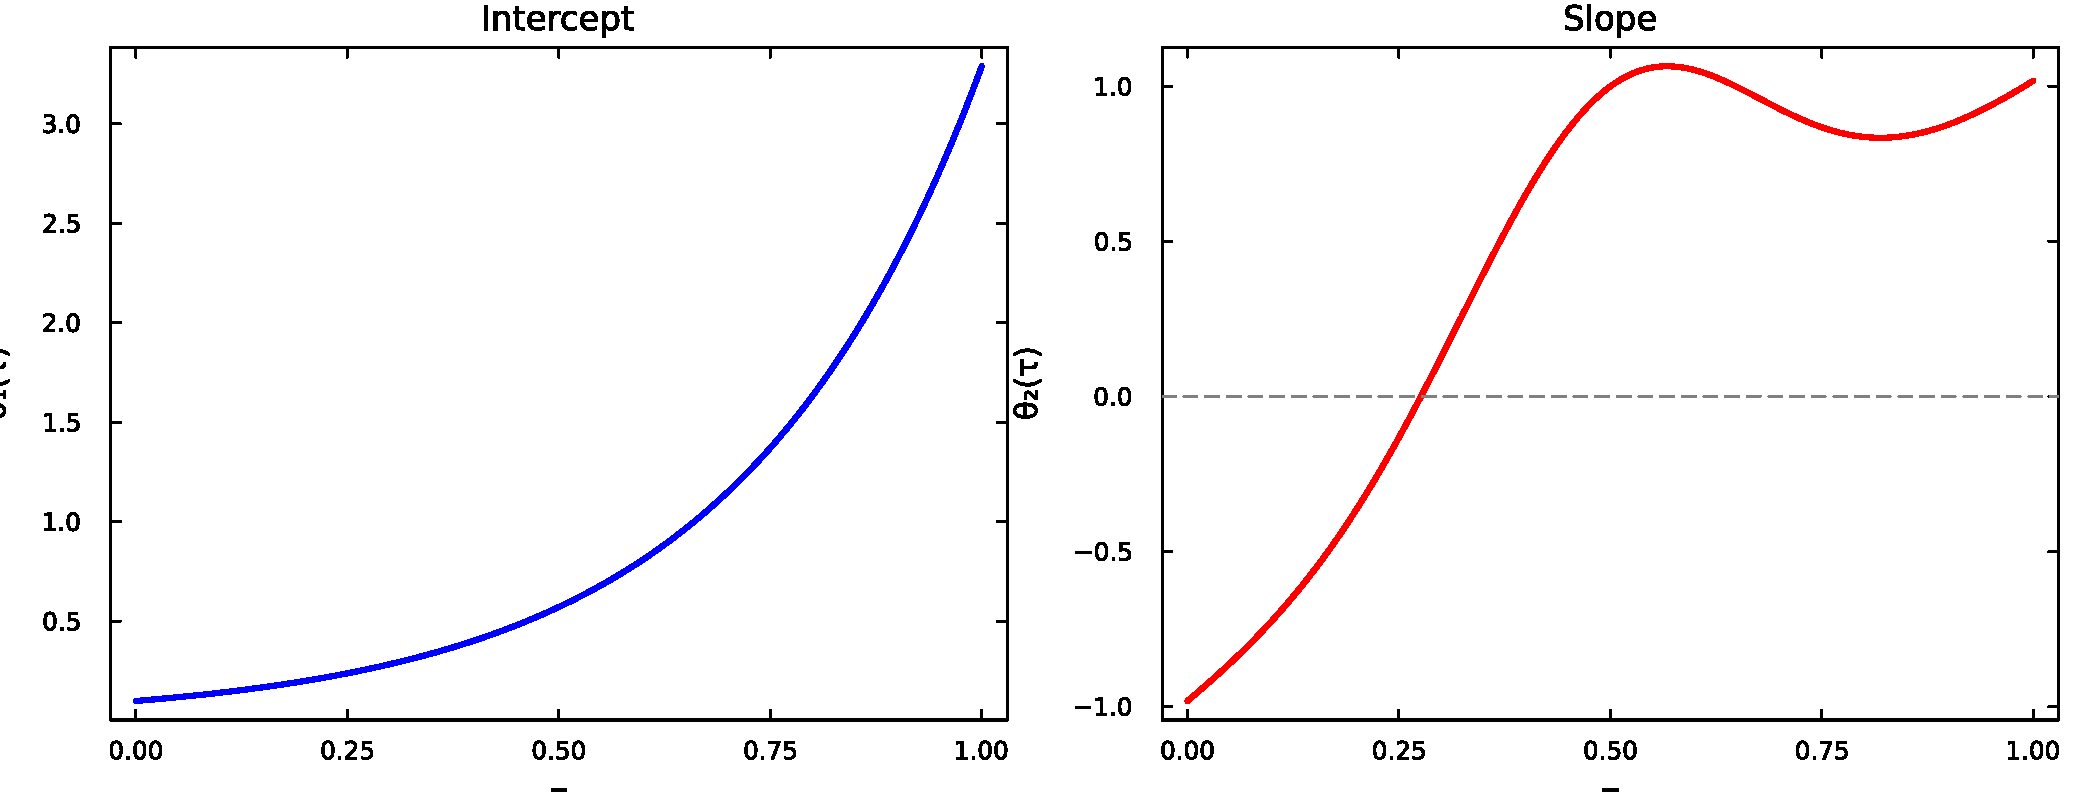
\includegraphics[width=0.9\textwidth]{theta_paths.pdf}
\caption{True parameter paths $\theta_1(\tau)$ and $\theta_2(\tau)$ for the Monte Carlo designs.}
\label{fig:theta-paths}
\end{figure}

\emph{Design~2} tests the estimator under a harder identification environment: a single instrument $Z_t \sim \mathrm{Unif}(-2, 2)$ enters a nonlinear, regime-switching first stage,
\[
  X_t = 10(2 S_t - 1)\bigl(Z_t - \tfrac{2}{5} Z_t^3\bigr) + v_t,
  \qquad
  S_t = \bigl[1 + e^{-(\tau - 1/4)(\tau - 3/4)\, T}\bigr]^{-1},
\]
in which the factor $(2 S_t - 1)$ flips sign across the regime boundaries at $\tau = 1/4$ and $\tau = 3/4$, so that the instrument's relevance for $X_t$ changes with $\tau$ and vanishes near the transitions. Figure~\ref{fig:design2} shows the resulting conditional mean $\E[X_t \mid Z_t]$ in each regime and the transition function $S(t)$ itself. 

\begin{figure}[H]
\centering
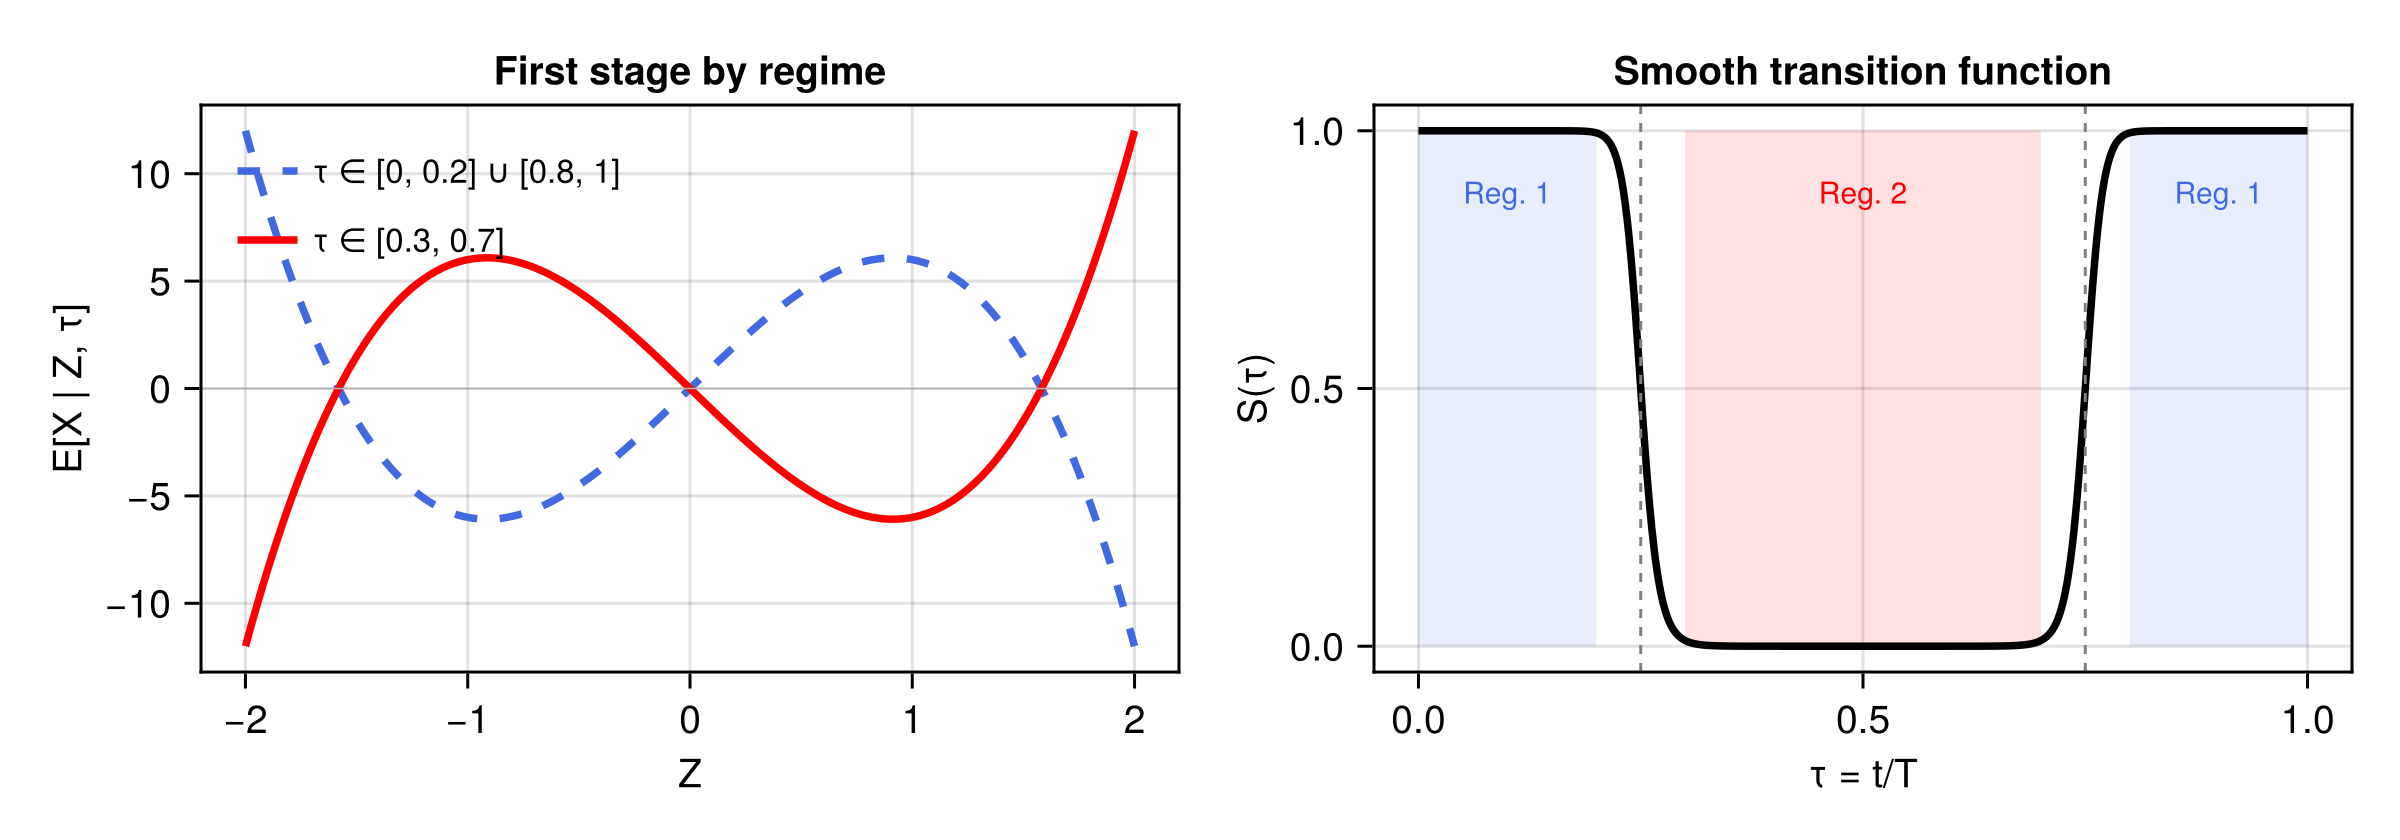
\includegraphics[width=0.85\textwidth]{design2_panels.png}
\caption{Design~2: the conditional mean of $X_t$ given $Z_t$ flips sign across regimes (left), governed by the smooth transition function $S(t)$ (right).}
\label{fig:design2}
\end{figure}

Both designs use $R = 1{,}000$ Monte Carlo replications at each sample size $T \in \{200, 400, 800\}$, one iteration of the Gao-Tsay bias correction, and $B = 1{,}000$ multiplier-bootstrap draws for the simultaneous confidence band. Tables~\ref{tab:mc} and~\ref{tab:mc-str} report the natural linear spline estimator; Table~\ref{tab:ncs-mc} adds the natural cubic spline counterpart. The regularization parameter $\lambda$ is selected separately in each replication by leave-one-out cross-validation (LOOCV): letting $\mathbf{H}_\lambda = \bfD\bfS_\lambda$ denote the hat matrix that maps $\bfy$ to the fitted values $\bfD\hat\btheta$, the selector minimises $T^{-1}\sum_i\bigl((y_i - \hat y_i)/(1 - [\mathbf{H}_\lambda]_{ii})\bigr)^2$ over a log-spaced grid of $\lambda$.

\subsection{Design~1: four instruments, linear first stage}

Table~\ref{tab:mc} reports the bias-corrected estimator's Design~1 summary.

\begin{table}[H]
\centering
\caption{Design~1 (LZH, $p = 2$), natural linear spline estimator: Monte Carlo summary, $R = 1{,}000$ replications. All columns averaged over the interior $[0.05, 0.95]$ and over replications. \emph{PW}: $95\%$ pointwise coverage rate (averaged over $\tau$ and reps). \emph{SCB}: fraction of replications in which the $95\%$ simultaneous band contains $\theta_0(\tau)$ at every interior $\tau$.}
\label{tab:mc}
\small
\begin{tabular}{@{}ll rrrr rr@{}}
\toprule
& & \multicolumn{4}{c}{Estimation} & \multicolumn{2}{c}{Coverage} \\
\cmidrule(lr){3-6}\cmidrule(lr){7-8}
$T$ & & Avg MSE & Avg Bias & Avg Var & Avg MAD & PW & SCB \\
\midrule
\multirow{2}{*}{200}
& $\theta_1$ & .0645 & $+$.0263 & .0585 & .2016 & .907 & .800 \\
& $\theta_2$ & .0154 & $+$.0087 & .0151 & .0965 & .920 & .737 \\
\midrule
\multirow{2}{*}{400}
& $\theta_1$ & .0529 & $+$.0200 & .0484 & .1816 & .919 & .863 \\
& $\theta_2$ & .0123 & $+$.0067 & .0121 & .0861 & .936 & .838 \\
\midrule
\multirow{2}{*}{800}
& $\theta_1$ & .0445 & $+$.0170 & .0413 & .1672 & .932 & .903 \\
& $\theta_2$ & .0096 & $+$.0042 & .0096 & .0760 & .952 & .924 \\
\bottomrule
\end{tabular}
\end{table}

MSE and MAD decrease monotonically with $T$, variance dominates squared bias at every cell, and both pointwise and simultaneous coverage rise toward nominal, with the latter rising more slowly because the band must hold uniformly over $\tau$. LOOCV selects a rescaled $\lambda T^{2/3}$ that grows from roughly $0.38$ at $T = 200$ to $0.71$ at $T = 800$, slightly slower shrinkage than the IMSE-optimal $T^{-2/3}$ rate. 

Figure~\ref{fig:per-tau-mse} shows the per-$\tau$ MSE converging toward zero across the interior as $T$ grows, with the largest levels at the boundaries of $[0,1]$ (standard for penalised smoothers) and at the high-curvature regions of the true functions. As it is visible in the figure \ref{fig:per-tau-mse}, the estimator is more successful at tracking the slope $\theta_2$ than the intercept $\theta_1$ in terms of MSE.
\begin{figure}[H]
\centering

\includegraphics[width=0.95\textwidth]{lzh_per_tau_mse.pdf}
\caption{Design~1, natural linear spline estimator: pointwise MSE as a function of $\tau$. Solid: $T = 200$. Dashed: $T = 400$. Dotted: $T = 800$.}
\label{fig:per-tau-mse}
\end{figure}


\subsection{Design~2: one instrument, nonlinear first stage}

Design~2 puts the estimator under stress through regime change in the non-linear first stage: at the regime transitions $\tau = 0.25$ and $\tau = 0.75$ the first stage is specification changes dramatically and the challenge for estimator is to accomodate this non-linearity without specifying any parametrization of true specification of first stage. Table~\ref{tab:mc-str} shows how this affects Monte Carlo performance.

\begin{table}[H]
\centering
\caption{Design~2 (STR, $p = 2$), natural linear spline estimator: Monte Carlo summary, $R = 1{,}000$ replications. Column definitions as in Table~\ref{tab:mc}.}
\label{tab:mc-str}
\small
\begin{tabular}{@{}ll rrrr rr@{}}
\toprule
& & \multicolumn{4}{c}{Estimation} & \multicolumn{2}{c}{Coverage} \\
\cmidrule(lr){3-6}\cmidrule(lr){7-8}
$T$ & & Avg MSE & Avg Bias & Avg Var & Avg MAD & PW & SCB \\
\midrule
\multirow{2}{*}{200}
& $\theta_1$ & .0342 & $+$.0164 & .0328 & .1455 & .887 & .693 \\
& $\theta_2$ & .0078 & $+$.0331 & .0064 & .0694 & .792 & .141 \\
\midrule
\multirow{2}{*}{400}
& $\theta_1$ & .0200 & $+$.0088 & .0196 & .1119 & .920 & .820 \\
& $\theta_2$ & .0048 & $+$.0306 & .0038 & .0550 & .829 & .199 \\
\midrule
\multirow{2}{*}{800}
& $\theta_1$ & .0129 & $+$.0065 & .0127 & .0899 & .933 & .892 \\
& $\theta_2$ & .0035 & $+$.0319 & .0024 & .0472 & .830 & .221 \\
\bottomrule
\end{tabular}
\end{table}

The intercept $\theta_1$ behaves as in Design~1, MSE falling and coverage rising with $T$, because its identification does not rely on instrument relevance. The slope $\theta_2$ shows a pattern the bias correction cannot fix: signed bias stays roughly constant across $T$ while the variance shrinks, so simultaneous-band coverage for $\theta_2$ stays far below nominal and pointwise coverage fails to converge. 

Figure~\ref{fig:str-mse} shows MSE for $\theta_2$ peaking at the regime transitions $\tau \approx 0.25$ and $\tau \approx 0.75$ where the instrument's regime changes. These peaks shrink with $T$ and as $T = 800$ they are not visible anymore.

\begin{figure}[H]
\centering

\includegraphics[width=0.95\textwidth]{str_per_tau_mse.pdf}
\caption{Design~2, natural linear spline estimator: per-$\tau$ MSE. The peaks for $\theta_2$ at $\tau \approx 0.25, 0.75$ mark the regime transitions where the instrument's local relevance vanishes.}
\label{fig:str-mse}
\end{figure}

In figure~\ref{fig:median-rep-m1}, we plot the median-MSE replication paths for Design~1, which are representative of the typical performance across replications. The bias-corrected estimates track the true paths well across the interior and the boundary effect seems to be minimal.  The paths stay relatively smooth with wiggles at different values of $T$, consistent with the natural linear spline's penalty structure.
\begin{figure}[H]
\centering

\includegraphics[width=0.95\textwidth]{lzh_median_rep_T200.pdf}\\[0.3em]

\includegraphics[width=0.95\textwidth]{lzh_median_rep_T400.pdf}\\[0.3em]

\includegraphics[width=0.95\textwidth]{lzh_median_rep_T800.pdf}
\caption{Design~1, natural linear spline estimator: median-MSE replication at $T = 200$ (top), $400$ (middle), and $800$ (bottom). Black: true $\theta_0(\tau)$. Blue: bias-corrected estimate. Black dashed: $95\%$ pointwise CI. Red dotted: $95\%$ SCB.}
\label{fig:median-rep-m1}
\end{figure}


\subsection{Natural cubic spline: head-to-head comparison}\label{sec:mc-ncs}

We rerun the same two designs using the natural cubic spline estimator; sample sizes, replication count, bootstrap design, $\lambda$-selection procedure, and interior grid are identical. Table~\ref{tab:ncs-mc} reports the same quantities as Tables~\ref{tab:mc} and~\ref{tab:mc-str}, directly comparable entry by entry.

\begin{table}[H]
\centering
\caption{Natural cubic spline estimator: Monte Carlo summary, $R = 1{,}000$ replications. All columns averaged over the interior $[0.05, 0.95]$ and over replications. \emph{PW}: $95\%$ pointwise coverage rate (averaged over $\tau$ and reps). \emph{SCB}: fraction of replications in which the $95\%$ simultaneous band contains $\theta_0(\tau)$ at every interior $\tau$.}
\label{tab:ncs-mc}
\small
\begin{tabular}{@{}l r rrrrr rr@{}}
\toprule
Design & $T$ & $\theta$ & MSE & Bias & Var & MAD & PW & SCB \\
\midrule
\multirow{6}{*}{LZH}
 & \multirow{2}{*}{200} & $\theta_1$ & .0646 & $+$.0028 & .0638 & .2004 & .934 & .916 \\
 &                      & $\theta_2$ & .0095 & $+$.0132 & .0090 & .0762 & .919 & .842 \\
 & \multirow{2}{*}{400} & $\theta_1$ & .0514 & $+$.0007 & .0504 & .1771 & .945 & .935 \\
 &                      & $\theta_2$ & .0069 & $+$.0101 & .0066 & .0647 & .935 & .899 \\
 & \multirow{2}{*}{800} & $\theta_1$ & .0403 & $+$.0032 & .0398 & .1568 & .952 & .952 \\
 &                      & $\theta_2$ & .0047 & $+$.0066 & .0046 & .0533 & .957 & .954 \\
\midrule
\multirow{6}{*}{STR}
 & \multirow{2}{*}{200} & $\theta_1$ & .0610 & $+$.0035 & .0609 & .1916 & .936 & .861 \\
 &                      & $\theta_2$ & .0072 & $+$.0356 & .0058 & .0663 & .886 & .605 \\
 & \multirow{2}{*}{400} & $\theta_1$ & .0367 & $-$.0010 & .0367 & .1489 & .952 & .917 \\
 &                      & $\theta_2$ & .0043 & $+$.0319 & .0033 & .0521 & .898 & .667 \\
 & \multirow{2}{*}{800} & $\theta_1$ & .0251 & $+$.0006 & .0250 & .1225 & .954 & .934 \\
 &                      & $\theta_2$ & .0033 & $+$.0331 & .0022 & .0461 & .878 & .593 \\
\bottomrule
\end{tabular}
\end{table}

Table~\ref{tab:ncs-mc} differs from the natural linear spline tables and Figure~\ref{fig:median-rep-m1} on three fronts: simultaneous-band coverage reaches nominal, the residual bias vanishes at the variance rate, and replication paths stay smooth as $T$ grows. The null space $\{1,\tau\}$ absorbs the linear component of the Design~1 exponential intercept without shrinkage, cutting its bias by nearly an order of magnitude; and the faster $T^{-4/5}$ rate shows through as a $38$–$51\%$ MSE reduction on $\theta_2$. On Design~2 the slope's simultaneous coverage improves three- to four-fold over the natural linear spline but stays below nominal, and the bootstrap variance ratio tightens to $[0.95, 1.04]$ across every cell against values as low as $0.74$ for the natural linear spline on Design~2 at $T = 200$.

Figure~\ref{fig:ncs-median-rep} shows the median-MSE replication under the natural cubic spline at each $T$. The estimate is smooth at every sample size, and the smoothness does not deteriorate with $T$.

\begin{figure}[H]
\centering
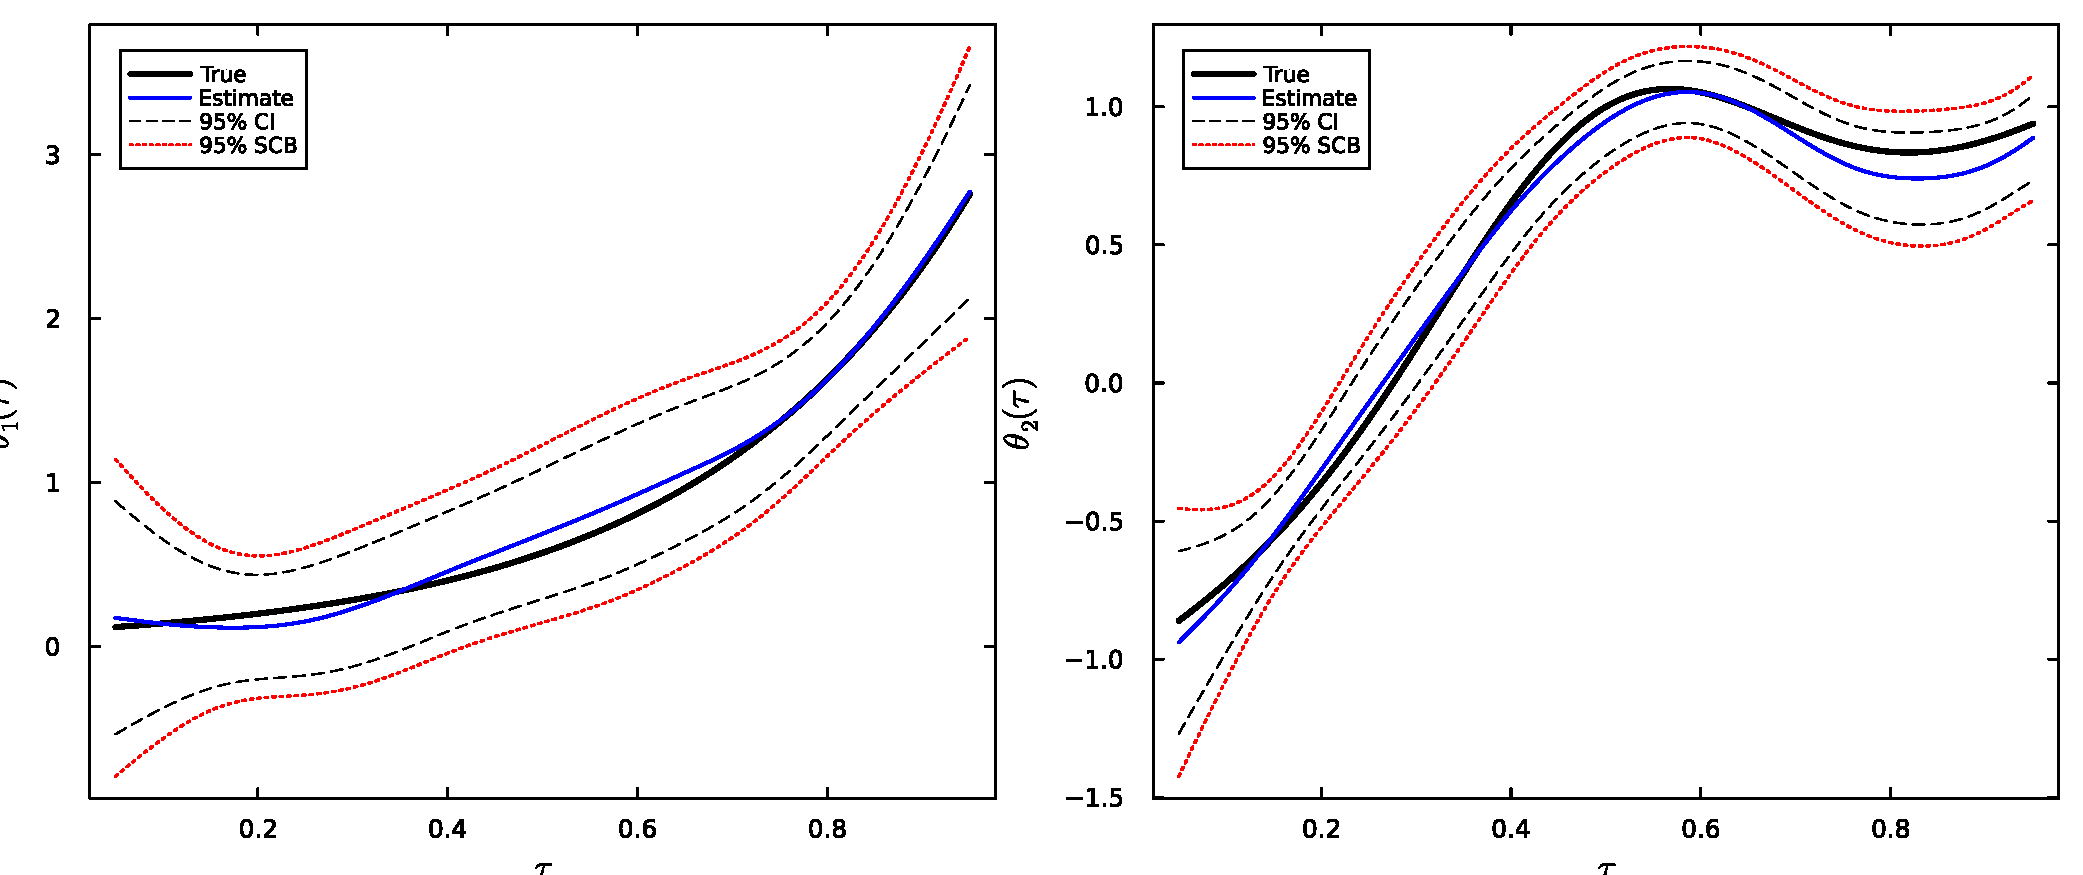
\includegraphics[width=0.9\textwidth]{figures/mc_ncs/lzh_median_rep_T200.pdf}\\[0.3em]
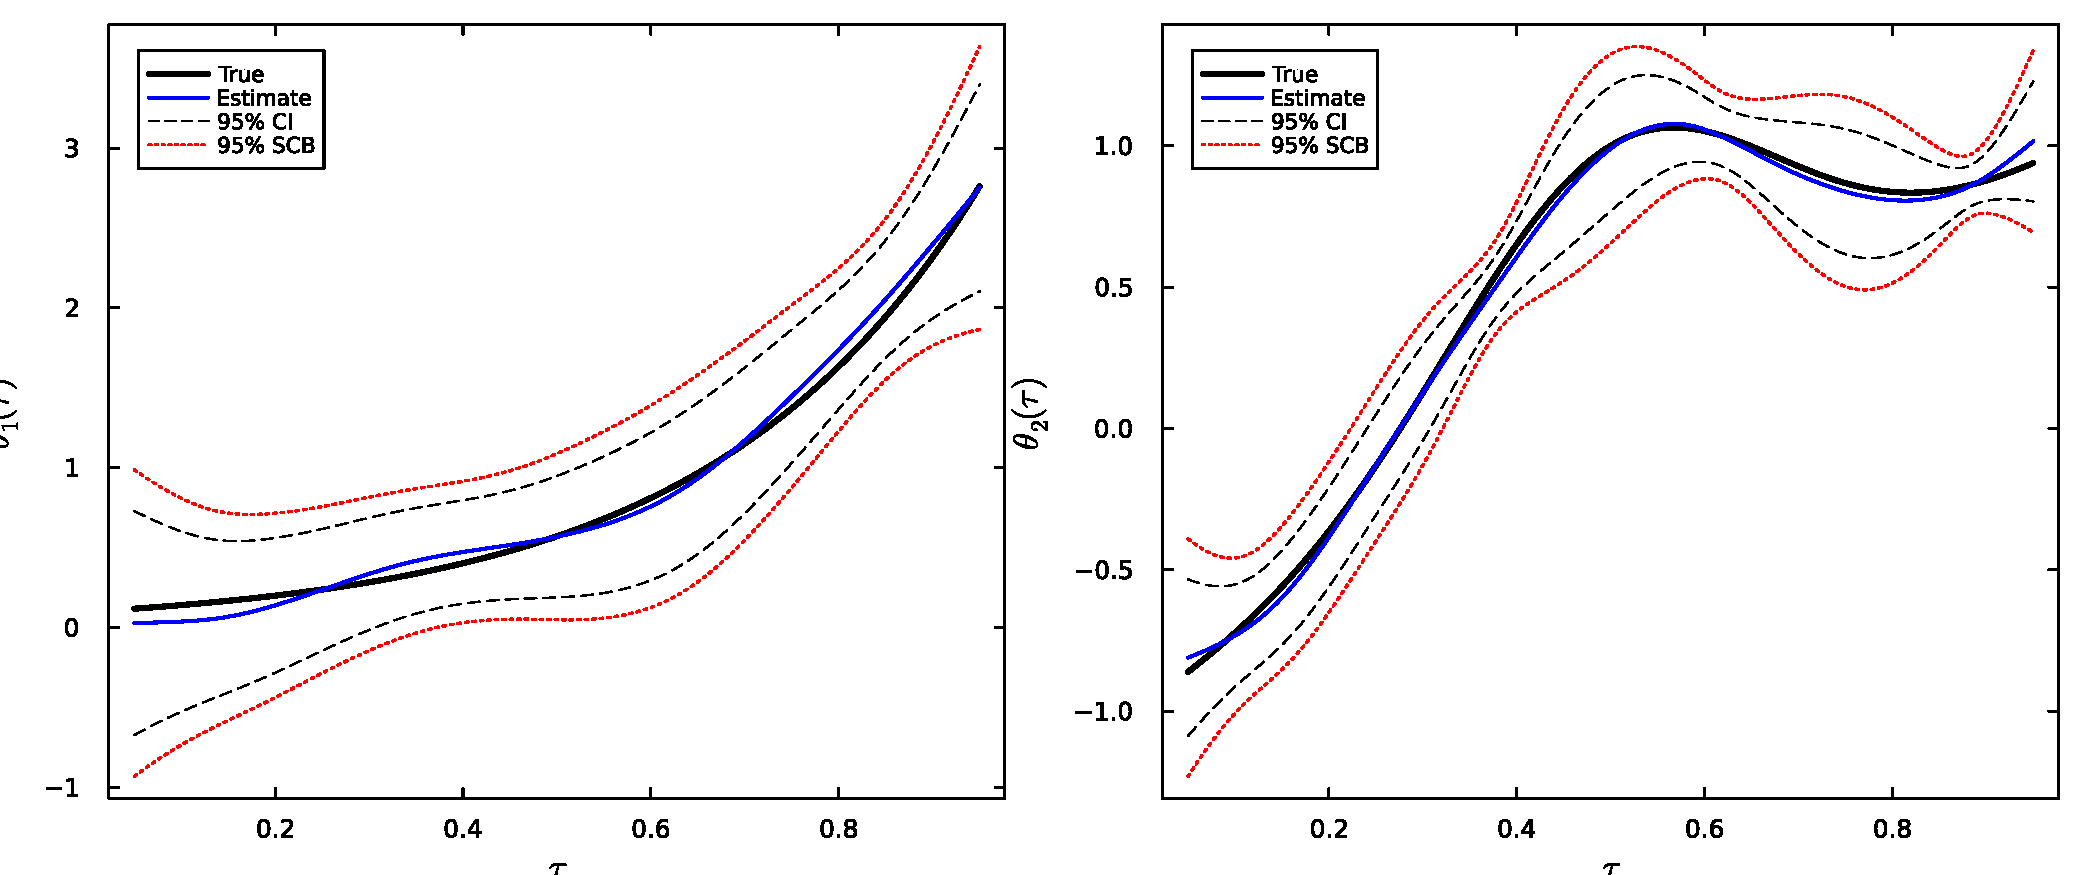
\includegraphics[width=0.9\textwidth]{figures/mc_ncs/lzh_median_rep_T400.pdf}\\[0.3em]
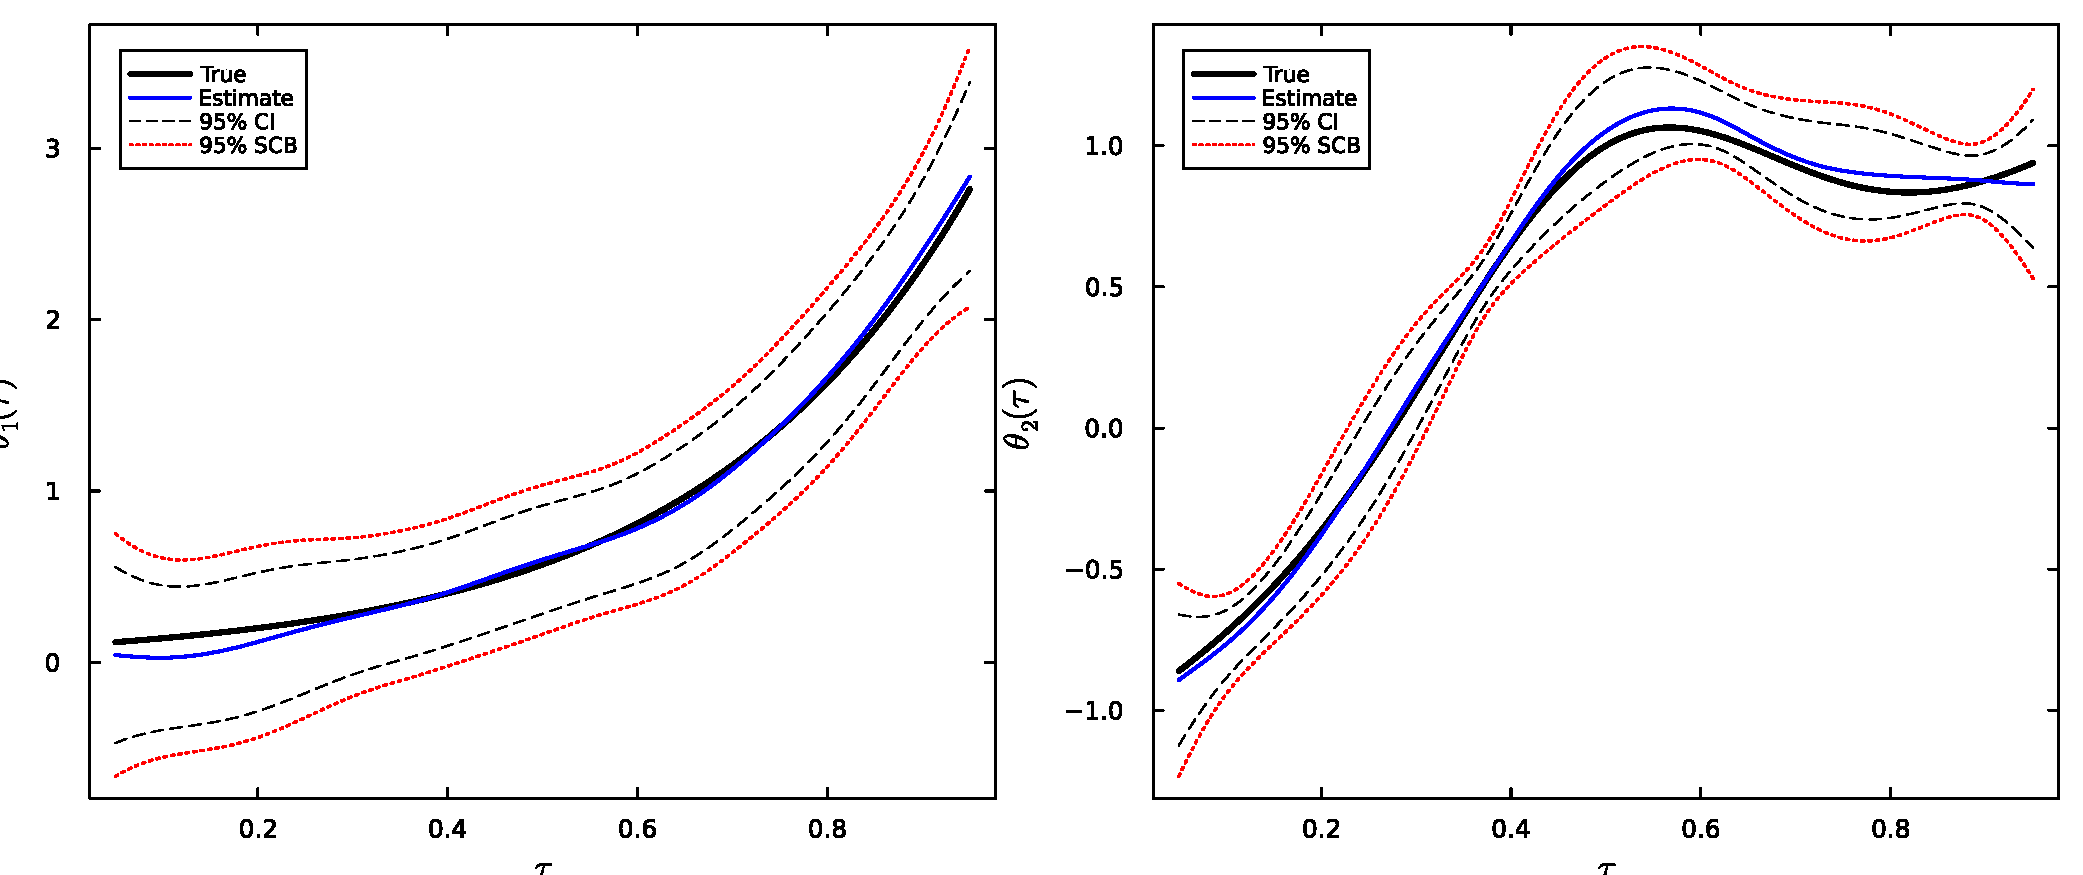
\includegraphics[width=0.9\textwidth]{figures/mc_ncs/lzh_median_rep_T800.pdf}
\caption{Design~1, natural cubic spline estimator: median-MSE replication at $T = 200$ (top), $400$ (middle), and $800$ (bottom). Black: true $\theta_0(\tau)$. Blue: bias-corrected estimate. Black dashed: $95\%$ pointwise CI. Red dotted: $95\%$ SCB.}
\label{fig:ncs-median-rep}
\end{figure}

Figures~\ref{fig:ncs-per-tau-mse} and~\ref{fig:ncs-per-tau-mse-str} show per-$\tau$ MSE. On Design~1 and ~2 the error shrinks uniformly in $\tau$ as $T$ grows.

\begin{figure}[H]
\centering
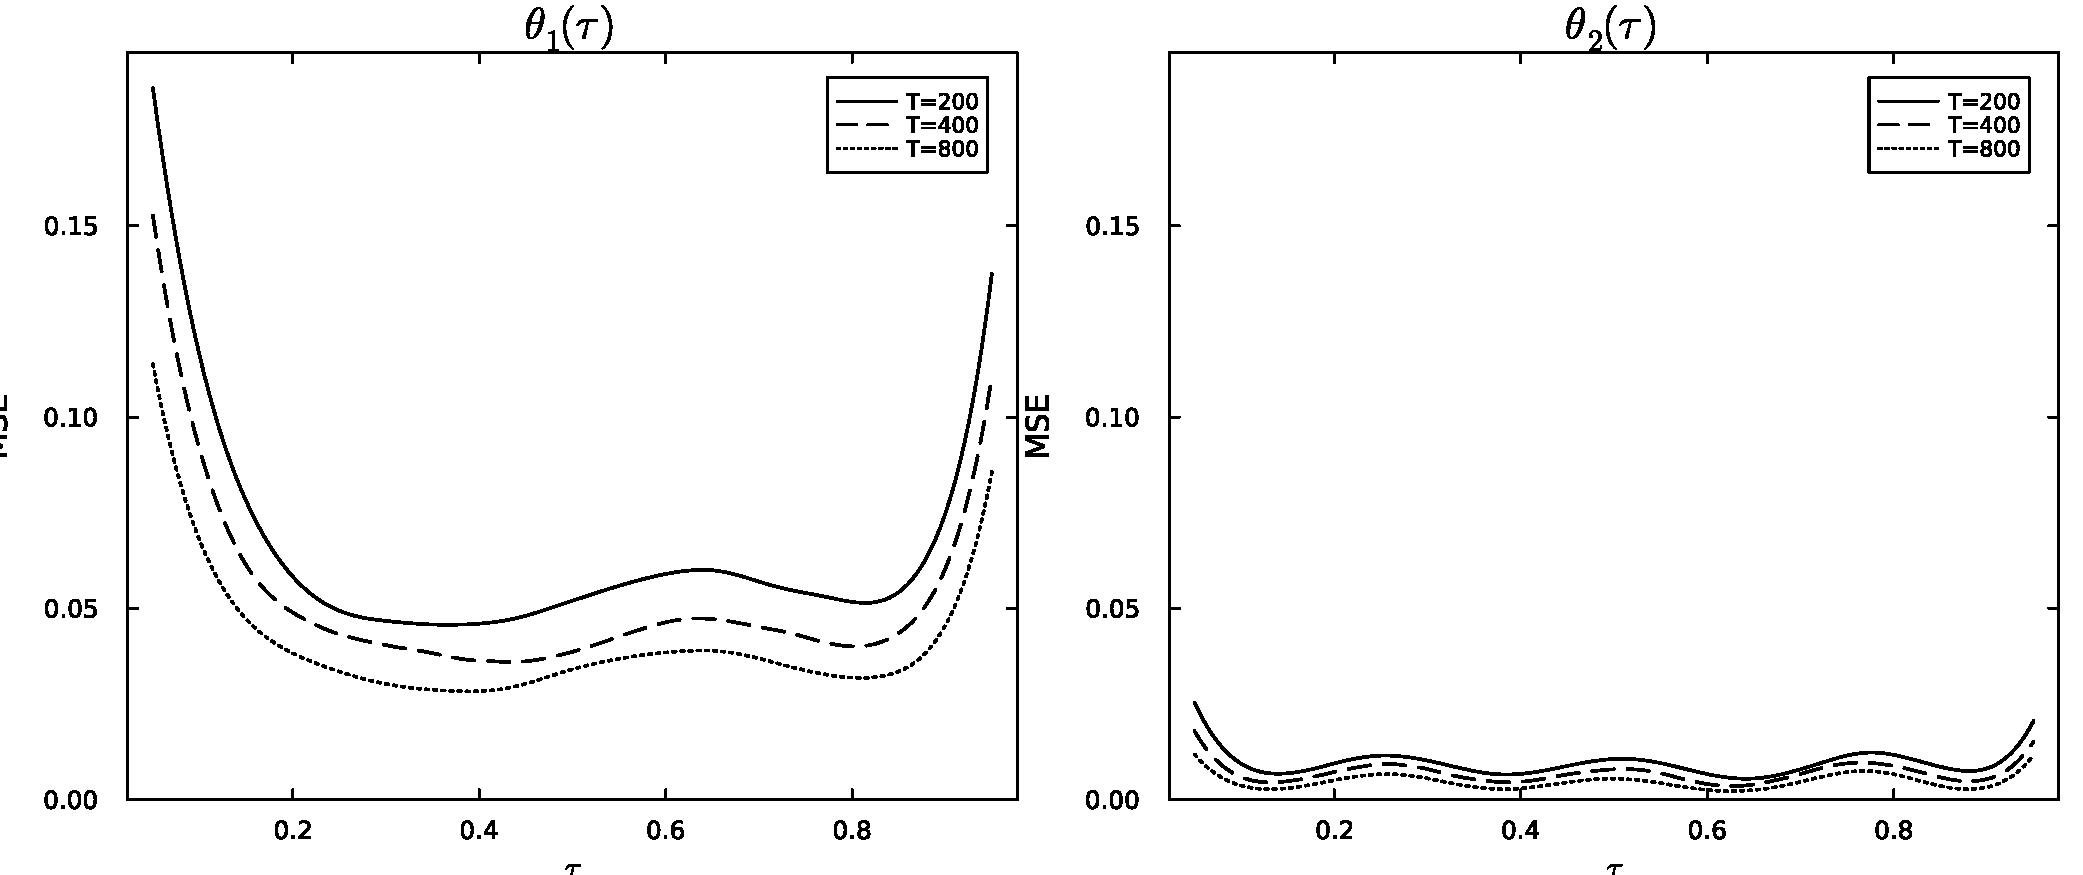
\includegraphics[width=0.95\textwidth]{figures/mc_ncs/lzh_per_tau_mse.pdf}
\caption{Design~1, natural cubic spline estimator: pointwise mean-squared error as a function of $\tau$. Solid: $T = 200$. Dashed: $T = 400$. Dotted: $T = 800$.}
\label{fig:ncs-per-tau-mse}
\end{figure}

\begin{figure}[H]
\centering
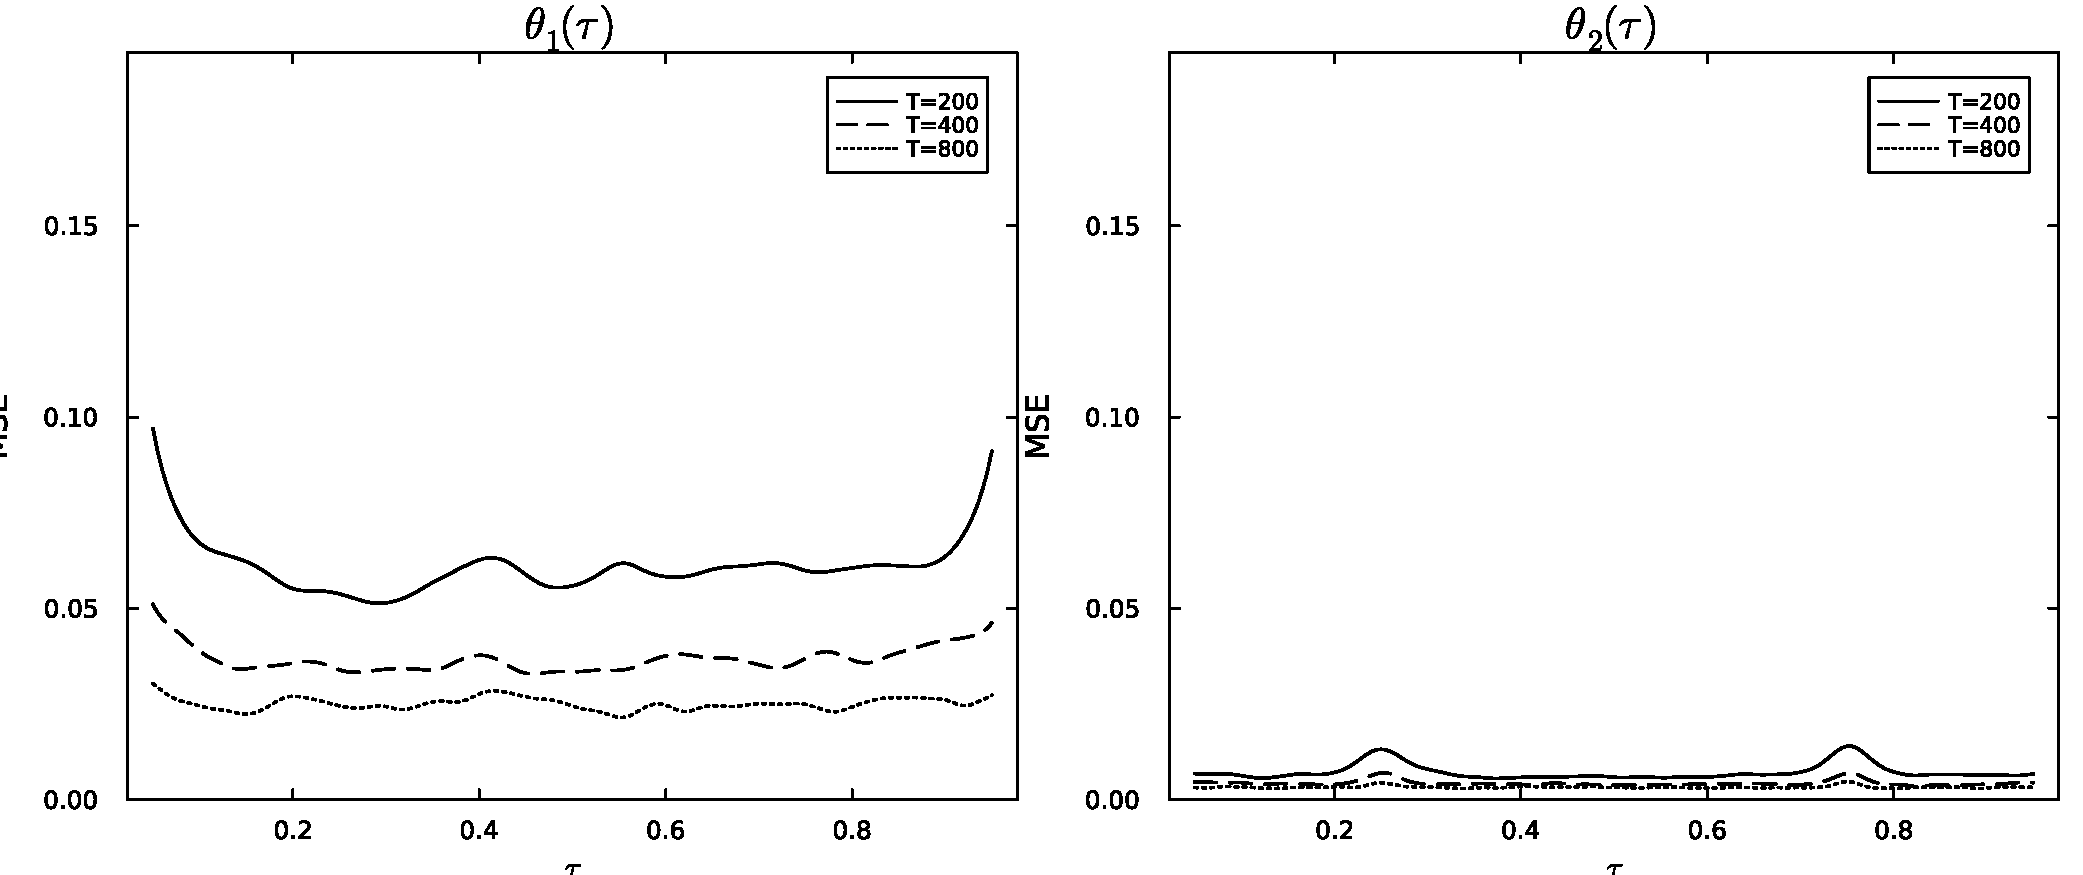
\includegraphics[width=0.95\textwidth]{figures/mc_ncs/str_per_tau_mse.pdf}
\caption{Design~2, natural cubic spline estimator: pointwise mean-squared error as a function of $\tau$. Solid: $T = 200$. Dashed: $T = 400$. Dotted: $T = 800$.}
\label{fig:ncs-per-tau-mse-str}
\end{figure}


\section{Empirical Application: The Phillips Curve Slope}\label{sec:nkpc}

Estimates of the unemployment slope of the aggregate U.S.\ Phillips curve have fallen sharply over the past half-century. \citet{StockWatson2019} put the slope at roughly $0.67$ over 1960 to 1983 and only $0.03$ over 2000 to 2019Q1, and \citet{Mavroeidis2014} show that this pattern survives reasonable variation in specification and sample. The standard interpretation reads the decline as a structural flattening of the Phillips curve since 1980, with the Volcker disinflation (a monetary contraction that produced large unemployment costs and a commensurate fall in inflation) as the cleanest remaining evidence of a once-steep slope.

\citet{Hazell2022} argue that this reading is wrong: the structural Phillips slope $\kappa$ was always small, and the apparent flattening is a statistical artifact of unmodeled shifts in long-run inflation expectations. Assume the unemployment gap $\tilde u_t$ follows an AR(1) with persistence $\rho_u$ and denote the household discount factor by $\beta$; solving the structural NKPC forward then gives the reduced form
\[
  \pi_t \;=\; -\psi\, \tilde u_t \;+\; E_t \pi_{t+\infty} \;+\; \omega_t, \qquad \psi \;=\; \frac{\kappa}{1-\beta \rho_u},
\]
where $\pi_t$ is inflation, $E_t \pi_{t+\infty}$ is long-run expected inflation, $\omega_t$ is a stationary residual, and the reduced-form slope $\psi$ scales the structural $\kappa$ by $1/(1-\beta\rho_u)$. Long-run expectations enter with coefficient one, so any regression omitting $E_t \pi_{t+\infty}$ projects regime shifts onto the unemployment slope. Over the Volcker period, when ten-year-ahead SPF CPI expectations fell from roughly $8\%$ to $4\%$ coincident with rising unemployment, the omitted-variable contamination creates a spurious steep slope in aggregate regressions. HHNS absorb $E_t \pi_{t+\infty}$ with time fixed effects in a state-level panel on U.S.\ non-tradeable CPI and recover $\hat\kappa \approx 0.006$ on the full 1978 to 2018 sample.

We ask whether aggregate data can replicate HHNS's conclusion when the NKPC coefficients are allowed to drift smoothly over time. The specification of \citet{GaliGertler1999} in first differences is
\begin{equation}\label{eq:nkpc}
  \Delta\pi_t \;=\; c(\tau) \;+\; \rho(\tau)\,\Delta\pi_{t+1} \;+\; \gamma(\tau)\,\Delta\pi_{t-1} \;+\; \alpha(\tau)\,\Delta u_t \;+\; \varepsilon_t, \qquad \tau = t/T.
\end{equation}
The time-varying intercept $c(\tau)$ absorbs low-frequency drift in the inflation target, the forward coefficient $\rho(\tau)$ absorbs short-horizon expectations through realised future inflation (endogenous and instrumented by lags), and $\alpha(\tau)$ is the object under test. We use monthly U.S.\ FRED data: core CPI (\texttt{CPILFESL}, 1958 to 2025, $T = 806$) as the aggregate inflation measure closest in spirit to HHNS's non-tradeable subindex, and the civilian unemployment rate (\texttt{UNRATE}). Endogeneity in $\Delta\pi_{t+1}$ and $\Delta u_t$ is handled by four lags each of $\Delta\pi$ and $\Delta u$; pointwise standard errors use Newey-West HAC with twelve monthly lags; the simultaneous band uses the block multiplier bootstrap of Section~\ref{sec:inference} with $B = 1{,}000$ draws and block length $m_b = \lfloor T^{1/3}\rfloor \approx 9$. We report both estimators: the natural cubic spline in Figure~\ref{fig:core-ncs-all} and the natural linear spline in Figure~\ref{fig:core-all}.

\begin{figure}[H]
\centering
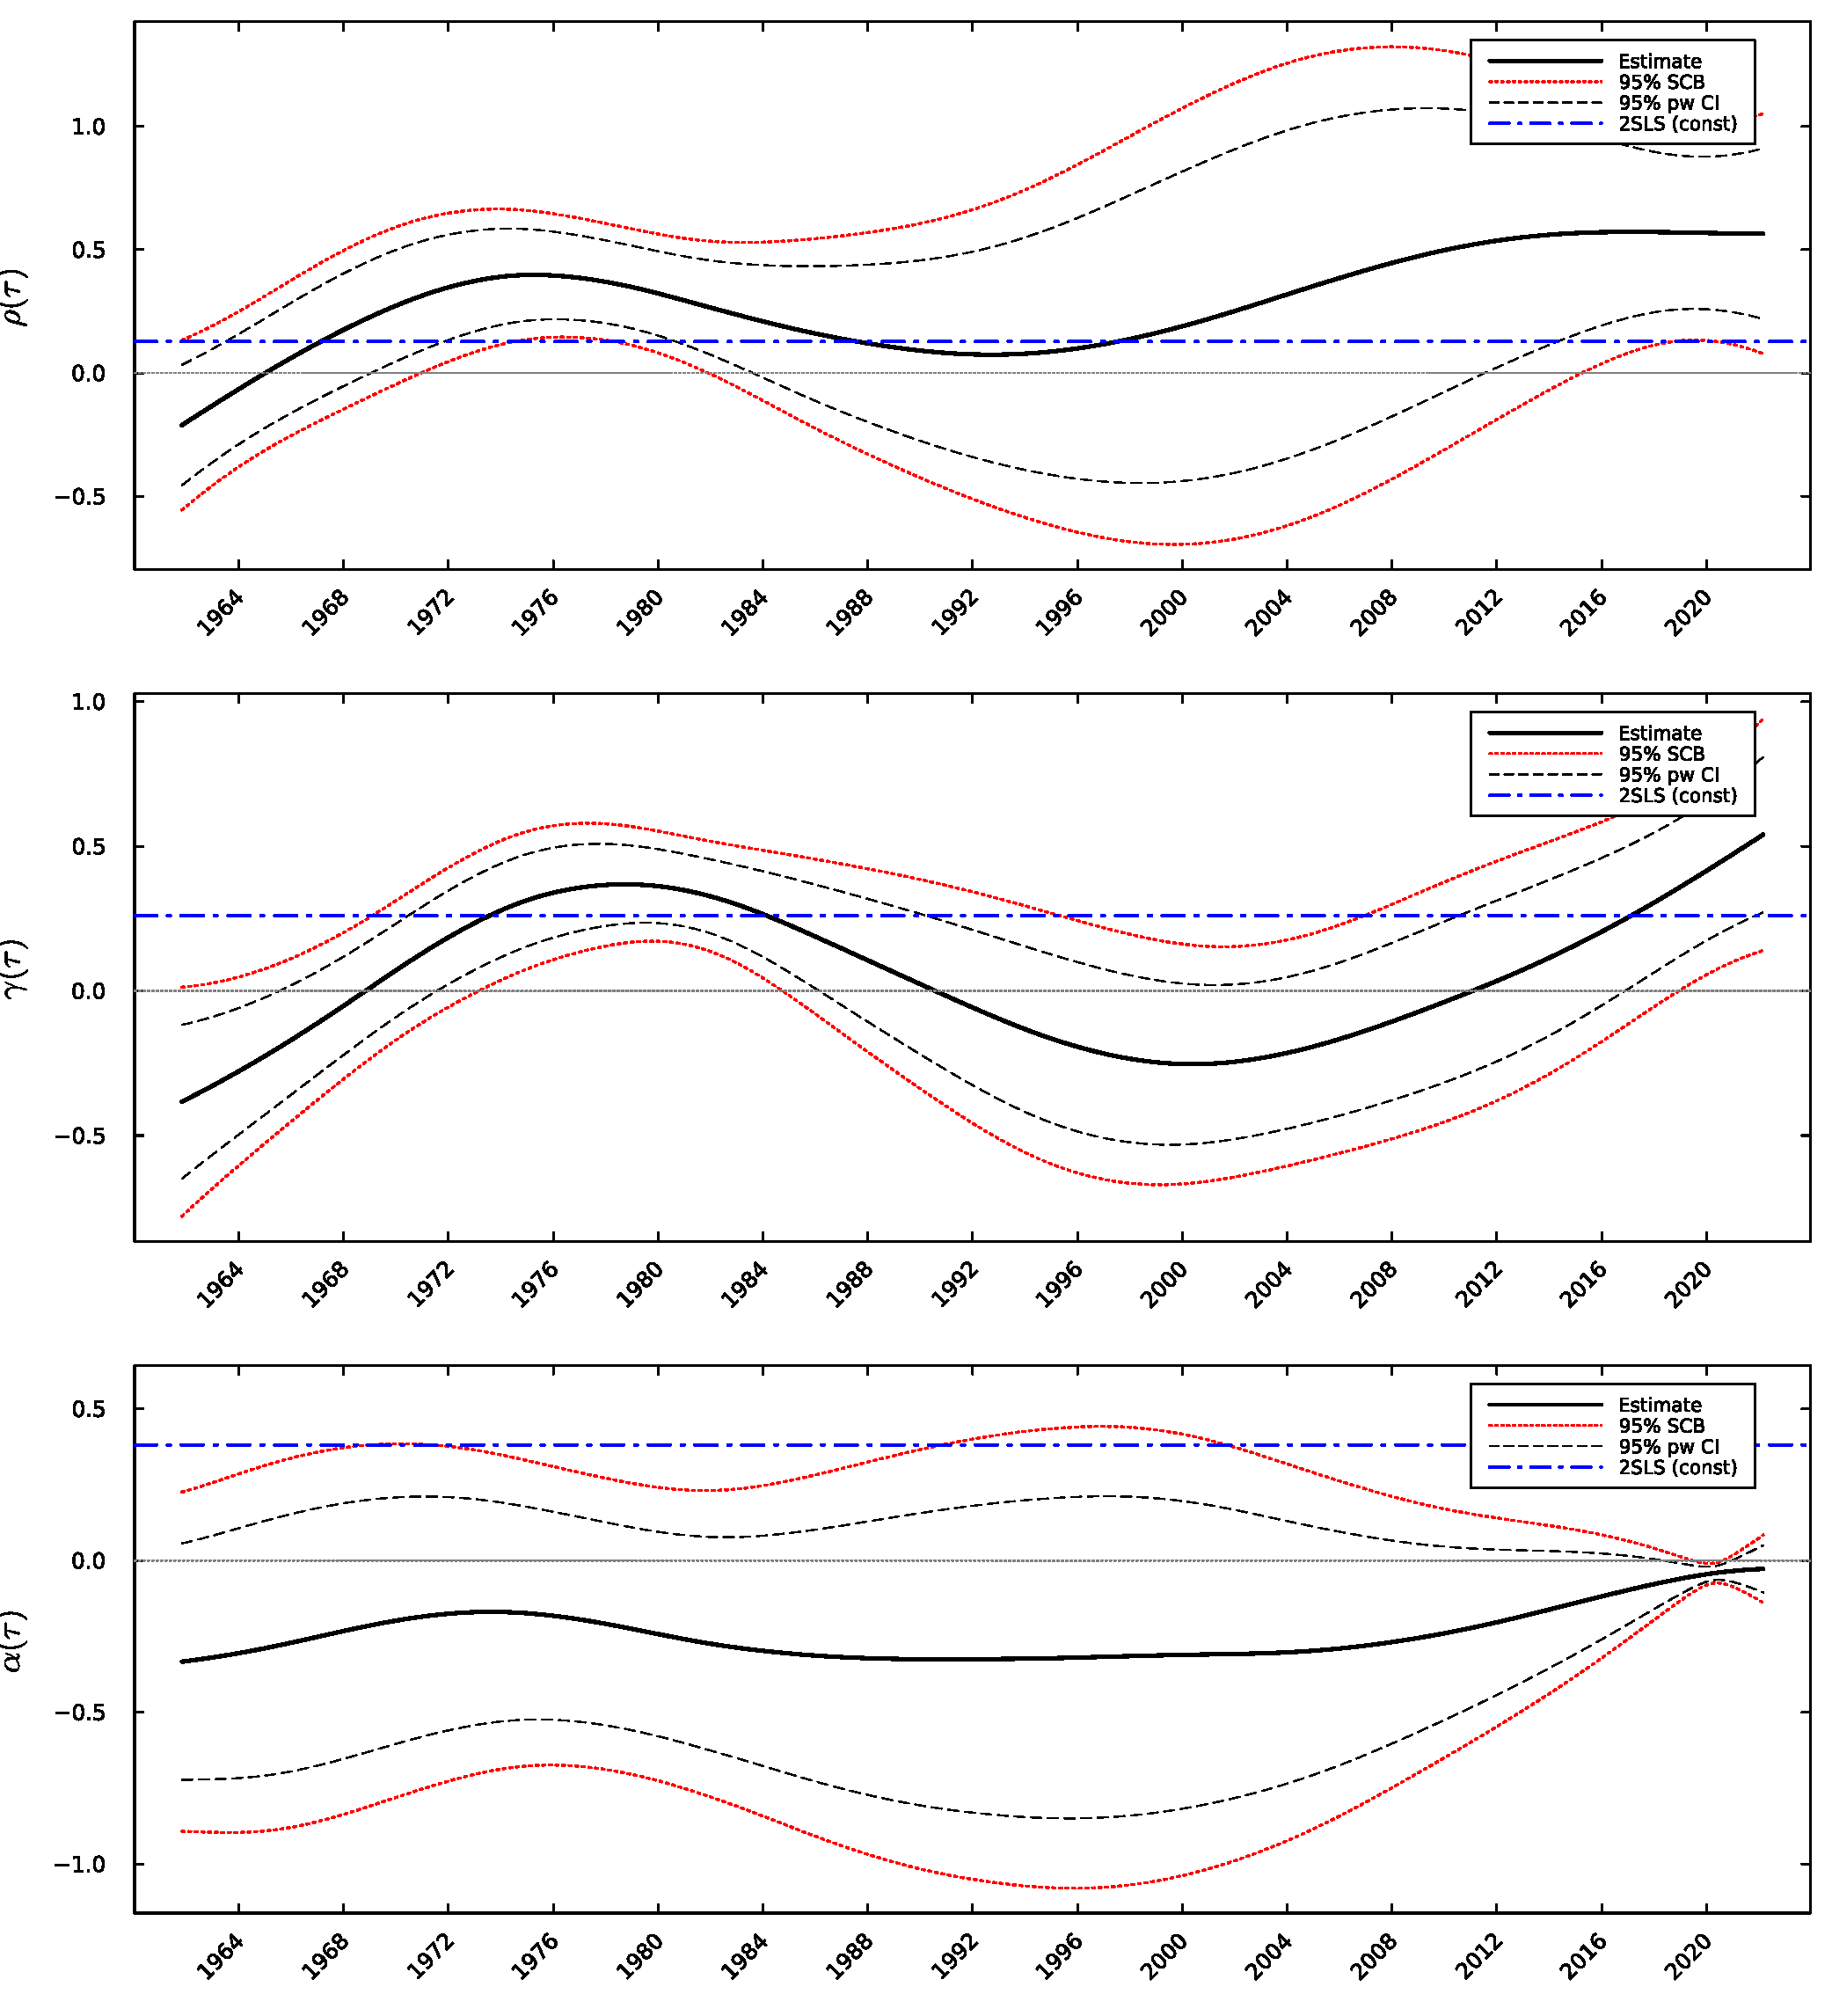
\includegraphics[width=0.95\textwidth]{results/nkpc_core_ncs/figures/nkpc_all_params.pdf}
\caption{Natural cubic spline estimator on core CPI, 1958 to 2025: forward-looking $\rho(\tau)$ (top), backward-looking $\gamma(\tau)$ (middle), Phillips slope $\alpha(\tau)$ (bottom). The intercept $c(\tau)$ is estimated but not plotted. Solid black: bias-corrected TVP estimate. Dashed black: $95\%$ pointwise HAC interval. Dotted red: $95\%$ simultaneous band. Blue dash-dot: constant-parameter 2SLS benchmark using the same eight instruments, $(\hat c, \hat\rho, \hat\gamma, \hat\alpha) = (0.19, 0.13, 0.26, 0.38)$. Y-axis ranges matched to Figure~\ref{fig:core-all}.}
\label{fig:core-ncs-all}
\end{figure}

Figure~\ref{fig:core-ncs-all} reports the three structural coefficient paths under the natural cubic spline estimator. The LOOCV-selected $\lambda$ is $3.4 \times 10^{-6}$, with residual standard deviation $\hat\sigma_\varepsilon = 0.214$ and $R^2 \approx 0.24$. All four coefficient paths reject constancy at the $5\%$ simultaneous level (the 2SLS benchmark lies outside the $95\%$ band on at least one interior interval), so the NKPC on U.S.\ core CPI is jointly time-varying over the sample.

The intercept $c(\tau)$ absorbs low-frequency drift in the inflation target, playing the role HHNS's time fixed effects play in their panel. The forward weight $\rho(\tau)$ and the backward weight $\gamma(\tau)$ both move from negative early in the sample to positive by the end, with intermediate fluctuations rather than a monotonic trajectory. This is what the HHNS identification story predicts: as long-run inflation expectations anchored post-Volcker, realised future inflation became a more stable and informative input to current inflation (hence $\rho$ rises on net), while the role of pure inflation persistence shifted from an unstable unit-root-like regime at the start of the sample toward a well-behaved AR(1)-like persistence by the end.

The Phillips slope $\alpha(\tau)$ is the object under test, and its pointwise $95\%$ CI contains zero across nearly the whole interior sample, with a single exception: the twelve-month window from June 2018 to December 2020, when U.S.\ unemployment reached its lowest level in fifty years. The 2SLS benchmark $\hat\alpha = 0.38$ lies outside the simultaneous band on most of the sample, so a constant slope is rejected; crucially, the rejection is toward zero rather than toward a steep pre-Volcker past.

Two further features sharpen the HHNS alignment. The post-pandemic 2021 to 2023 inflation surge does not register as a Phillips-curve activation: by the end of the sample the slope is within rounding of zero and its pointwise band contains zero throughout, contrary to the nonlinearity case of \citet{BenignoEggertsson2023} and \citet{Bernanke2023}. And the low-frequency drift in long-run SPF expectations between 1982 and 1998 is absorbed by the time-varying intercept and the rising forward weight, not by the slope.

Figure~\ref{fig:core-all} repeats the analysis with the natural linear spline estimator. The paths are less smooth than under the natural cubic spline but the qualitative conclusions are identical, so the findings are robust to the choice of estimator.

Two caveats bound these conclusions. First, instrumenting $\Delta\pi_{t+1}$ with lags is a short-horizon proxy for inflation expectations, not a direct substitute for HHNS's absorption of $E_t\pi_{t+\infty}$ via time fixed effects; the aggregate regression inherits the weak-instrument and imperfect-expectations-measure problems that \citet{Mavroeidis2014} emphasise. Second, the aggregate TVP specification does not escape the \citet{McLeayTenreyro2019} endogeneity problem that the regional design is built to solve.

\begin{figure}[H]
\centering

\includegraphics[width=0.95\textwidth]{nkpc_all_params.pdf}
\caption{Natural linear spline estimator on core CPI, 1958 to 2025. Panels and overlays as in Figure~\ref{fig:core-ncs-all}.}
\label{fig:core-all}
\end{figure}



\section{Conclusion}\label{sec:conclusion}

We developed two penalized SMD estimators for time-varying coefficient regression under endogeneity (a natural linear spline and a natural cubic spline), sharing a common instrument kernel, a Gao-Tsay bias correction, and a multiplier-bootstrap simultaneous confidence band. Monte Carlo evidence documents the finite-sample behaviour of each estimator with complementary trade-offs across strongly and locally-weakly identified designs.

On U.S.\ core-CPI Phillips-curve data both estimators deliver the same conclusion: the unemployment slope is pointwise indistinguishable from zero across nearly the whole interior sample, with a single narrow window in the 2018 to 2020 tight-labor-market episode, consistent with \citet{Hazell2022}'s claim that the apparent flattening of the aggregate Phillips curve is driven by long-run-expectations drift rather than by a structural change in the slope.

Natural extensions include addressing the local weak-instrument problem and broadening the framework so that the functional parameter is indexed by an economically meaningful variable other than rescaled time, such as age, income, or market concentration.

All figures and estimates are produced by the accompanying Julia package \texttt{TVPSobolev.jl}; three driver scripts regenerate every result from \texttt{data/} inputs under a fixed seed.


\begin{thebibliography}{20}

\bibitem[Antoine and Shahryarpoor(2024)]{AntoineShahryarpoor}
Antoine, B.\ and Shahryarpoor, F.\ (2024).
\newblock Robust estimation in conditional moment models with time-varying parameters.
\newblock Working paper, Simon Fraser University.

\bibitem[Antoine and Sun(2024)]{AntoineSun2024}
Antoine, B.\ and Sun, Y.\ (2024).
\newblock Smooth minimum distance estimation for dependent data.
\newblock \emph{Journal of Financial Econometrics}, forthcoming.

\bibitem[Benigno and Eggertsson(2023)]{BenignoEggertsson2023}
Benigno, P.\ and Eggertsson, G.~B.\ (2023).
\newblock It's baaack: The surge in inflation in the 2020s and the return of the non-linear {P}hillips curve.
\newblock NBER Working Paper No.\ 31197.

\bibitem[Bernanke and Blanchard(2023)]{Bernanke2023}
Bernanke, B.~S.\ and Blanchard, O.\ (2023).
\newblock What caused the {U.S.} pandemic-era inflation?
\newblock Hutchins Center Working Paper No.\ 86, Brookings Institution.

\bibitem[Bierens(1982)]{Bierens1982}
Bierens, H.~J.\ (1982).
\newblock Consistent model specification tests.
\newblock \emph{Journal of Econometrics}, 20(1):105-134.

\bibitem[Eubank(1988)]{Eubank1988}
Eubank, R.~L.\ (1988).
\newblock \emph{Spline Smoothing and Nonparametric Regression}.
\newblock Marcel Dekker, New York.

\bibitem[Gal\'{i} and Gertler(1999)]{GaliGertler1999}
Gal\'{i}, J.\ and Gertler, M.\ (1999).
\newblock Inflation dynamics: A structural econometric analysis.
\newblock \emph{Journal of Monetary Economics}, 44(2):195-222.

\bibitem[Gao and Tsay(2024)]{GaoTsay2024}
Gao, J.\ and Tsay, R.~S.\ (2024).
\newblock Bias correction for nonparametric regression with time-varying coefficients.
\newblock Working paper.

\bibitem[Green and Silverman(1994)]{Green1994}
Green, P.~J.\ and Silverman, B.~W.\ (1994).
\newblock \emph{Nonparametric Regression and Generalized Linear Models: A Roughness Penalty Approach}.
\newblock Chapman \& Hall, London.

\bibitem[Kimeldorf and Wahba(1971)]{KimeldorfWahba1971}
Kimeldorf, G.\ and Wahba, G.\ (1971).
\newblock Some results on {T}chebycheffian spline functions.
\newblock \emph{Journal of Mathematical Analysis and Applications}, 33(1):82-95.

\bibitem[Hazell, Herre\~{n}o, Nakamura, and Steinsson(2022)]{Hazell2022}
Hazell, J., Herre\~{n}o, J., Nakamura, E., and Steinsson, J.\ (2022).
\newblock The slope of the {P}hillips curve: {E}vidence from {U.S.}\ states.
\newblock \emph{Quarterly Journal of Economics}, 137(3):1299-1344.

\bibitem[Mavroeidis, Plagborg-M{\o}ller, and Stock(2014)]{Mavroeidis2014}
Mavroeidis, S., Plagborg-M{\o}ller, M., and Stock, J.~H.\ (2014).
\newblock Empirical evidence on inflation expectations in the {N}ew {K}eynesian {P}hillips curve.
\newblock \emph{Journal of Economic Literature}, 52(1):124-188.

\bibitem[McLeay and Tenreyro(2019)]{McLeayTenreyro2019}
McLeay, M.\ and Tenreyro, S.\ (2019).
\newblock Optimal inflation and the identification of the {P}hillips curve.
\newblock \emph{NBER Macroeconomics Annual}, 34:199-255.

\bibitem[Stock and Watson(2019)]{StockWatson2019}
Stock, J.~H.\ and Watson, M.~W.\ (2019).
\newblock Slack and cyclically sensitive inflation.
\newblock NBER Working Paper No.\ 25987.

\bibitem[Wahba(1990)]{Wahba1990}
Wahba, G.\ (1990).
\newblock \emph{Spline Models for Observational Data}.
\newblock SIAM, Philadelphia.

\bibitem[Wu(2005)]{Wu2005}
Wu, W.~B.\ (2005).
\newblock Nonlinear system theory: Another look at dependence.
\newblock \emph{Proceedings of the National Academy of Sciences}, 102(40):14150-14154.

\bibitem[Zhou(2014)]{Zhou2014}
Zhou, Z.\ (2014).
\newblock Inference of weighted V-statistics for nonstationary time series and its applications.
\newblock \emph{Annals of Statistics}, 42(1):87-114.

\bibitem[Zhou and Wu(2009)]{Zhou2009}
Zhou, Z.\ and Wu, W.~B.\ (2009).
\newblock Local linear quantile estimation for nonstationary time series.
\newblock \emph{Annals of Statistics}, 37(5B):2696-2729.

\bibitem[Zhou and Wu(2010)]{ZhouWu2010}
Zhou, Z.\ and Wu, W.~B.\ (2010).
\newblock Simultaneous inference of linear models with time varying coefficients.
\newblock \emph{Journal of the Royal Statistical Society: Series B}, 72(4):513-531.

\end{thebibliography}

\end{document}
